% T8 of the Transport Papers series (consolidated).
% Correction (2026-09-10, mechanical pass, per Leon): rule 23 misidentified T5 as the printed-version exception. T1 is the exception at Version 3.0; every other paper, T5 included, reads Version 1.0. \date corrected accordingly (was 1.1).
% v1.1 (2026-09-10, derivation session, Fable 5.1 subagent, per rule 20,
%   series-review repair pass against series_review_2026-09-09.md).
%   Review 2.7: Prop 4.10 statement "whenever 4a notin Z" -> "whenever
%   a notin 6Z"; proof "unless 4a in Z, and is then irrational" -> 48^{a/6}
%   = 2^{2a/3} 3^{a/6} is rational exactly when a in 6Z, otherwise irrational,
%   with a = 3/2 giving 2 * 3^{1/4} as the example. Conclusion unchanged.
%   Sec 7 (Record/echo paragraph, review sec 3): "tens of milliseconds" ->
%   "tens to hundreds of milliseconds" with the figures 35 ms at 10 M_sun and
%   0.1 to 0.25 s at 30 to 70 M_sun (8M ln(M/m_P)); "A framework that commits
%   to an observational position is worth more than one that does not" ->
%   "The prediction is stated so that it can fail"; the GWTC-4.0 paragraph's
%   "which is the position a falsifiable framework should occupy" dropped.
%   \bibitem{ButlerT3} given T3's full subtitle. \date -> Version 1.1.
%   Thm 5.4's environment NOT changed. Abstract 249 words, unchanged.
%   Script: verify_T08.py 47/47. The Prop 4.10 irrationality check now tests
%   the correct condition: irrational at a = 1/4, 1/2, 3/4, 3/2, 3 (with the
%   value 2 * 3^{1/4} at a = 3/2 confirmed), rational at a = 0, 6, -6; the old
%   check listed 4a = 6 as irrational against its own "unless 4a in Z" label.
%   Count unchanged.
%   Compile: pdflatex x2, 23 pages, 0 errors, 0 undefined refs, 0 multiply
%   defined, 1 overfull, no float overflow.
%   Addendum 2026-09-09 (coordinator, same review-repair session): the ButlerT7
%   bibitem subtitle brought up to T7's current title ("State, Continuum, Lift,
%   and the Finite-Ledger Seam"). Bibliography only; nothing else changed.
% 2026-09-09 addendum (interactive session with Leon, Opus 5). Two changes
%   per Leon: (1) the printed version is now 1.0 for every paper T0 to T17,
%   T5 alone at 3.0 (progress-doc rule 23); the development numbering is
%   retired from the title page and kept in this header. (2) Every reference
%   to the programme monograph is removed (rule 24), re-pointed to the series
%   where a sibling paper carries the result and otherwise restated to stand
%   alone. No mathematics, no labels and no numbering changed, so verify_T08.py
%   stands unchanged at 47/47 and was not re-run.
%   Here: the family-faces principle is stated without attribution. NOTE: this
%   file was restored from the project copy in the same session after an
%   editing error truncated it; verified by structure and a clean compile.
% v1.10 (2026-09-08, derivation session, Fable 5.1 subagent, per rule 20,
%   review-repair pass against T08_review_v8.md).
%   Compile: 23pp, 0 errors, 0 warnings, 0 undefined refs, 0 multiply-defined,
%     1 overfull (6.44pt, cosmetic, left since v1.2), no float overflow;
%     verify_T08.py 47/47 (count unchanged: the tautological Prop 4.13
%     check replaced by one substantive check, the rationality closure of
%     the residue on 80 rules built from the paper's objects, formal in
%     ln 2; the transcendence of ln 2 is now stated as an import in
%     Section 10 and certified by no check). Numbering frozen: aux diff
%     empty on the sorted label map (Figure 1 now precedes Rem 4.6 in page order).
%   B1: Prop 4.10 retitled "Exactness excludes cutoff dependence", the
%     r_h / r_* = M dichotomy stated in it, "forced" replaced by "narrowed
%     to two scales" in the Section 4.1 opening, Rem 4.14, successor (1).
%   B2: the k = 0 / k != 0 split of Prop 4.13 carried into the opening,
%     Rem 4.14 and successor (1); the k != 0 exclusion moved from Proved
%     to Conditional in the levels list.  B3: as above.
%   S1 abstract count 47; S2 \date 1.10; S3 residue renamed kappa_c in
%     Props 4.12, 4.13, Rem 4.14, successor (1), script labels likewise;
%   S4 both yields as kappa_c = 4 pi (P1), 1 (P3) against 1/4, text and
%     script; S5 convention named at Contribution (2), the fence, Position
%     and coverage; S6 Prop 4.12 proof routed N_epoch/A via Cor 4.4(2);
%   S7 leading-order qualifier restored in Prop 4.8(i),(ii); S8 "real"
%     and "rational" a separated in Prop 4.10; S9 J3 flagged as modelling
%     in Fact 4.7, Rem 4.14's "closed" given its tier; S10 Kasner exponents
%     as proper-time exponents, (-1/2, 1, 1) in r; S11 rem:nu,
%     fact:capacity, the Position paragraph: calibration blocked behind
%     kappa_c and carried here; S12 T3 Prop 4.1 / Thm 4.2 cited.
%   N1, N2, N3 (Baker Thm 1.4), N6, N11, N13, N14, N16 done; the T6
%     admissible-class constraint sum p_i^2 = 1 noted in the 4.1 opening.
%   Knock-on noticed: T7 records no helicity successor problem (review).
%   Not done here (rule 20): milestone ticks, Run log, tp_status, sync.
% v1.9 (2026-09-08, prose pass, Fable 5.1 subagent, per project rule 22:
%   mannered prose replaced by literal statement, Leon's ruling to replace
%   the recurring vocabulary too). Body only; preamble title and bibitem
%   titles untouched. Compile: 22pp, 0 errors, 0 undefined refs,
%   0 multiply-defined; verify_T08.py 47/47 unchanged (three check-label
%   strings reworded, nothing else in the script); numbering unchanged
%   (aux diff empty on the sorted label map; Figure 1 keeps its number
%   but floats from p.10 to p.11, Section 4 running four lines longer).
%   Glossary applied: "ledger" (black-hole sense) -> "the boundary mode
%     space"/"the boundary modes" (66 sites, incl. Fact 2.1, Lem 4.2,
%     Prop 5.2 titles, Section 5 title, figure, caption); "window ledger"
%     -> "window mode space"; "the bet" -> "the prediction" (4, incl. Rem
%     4.14 title); "priced" -> "quantified" (2); "owns" -> "carries" (3);
%     "honest" dropped or -> "stated in full"/"declared"/"falsifiable" (4);
%     "The ledger of levels" -> "The levels of the results"; "wall
%     machinery" -> "wall results" (4); "touchpoint" -> "point of contact"
%     (2); "custody/business" -> "shared between/task"; "bookkeeping" ->
%     "computation" (2); "verdicts" -> "conclusions"; "lives at" -> "lies
%     at" (2); "faces/deploys" -> "instances/uses".
%   Non-glossary: "joints displayed" -> "step by step", "modelling joint"
%     -> "modelling step"; "blind(ness)" -> "insensitive/insensitivity";
%     "conveyor" -> "the window"; "cuts both ways" -> "holds in both
%     directions"; "breadcrumb" -> "identification"; "audited" ->
%     "examined"; "faced" -> "confronted"; "dead ends" -> "excluded routes".
% v1.8 (2026-09-07, derivation pass, gap-analysis fold-in of the
%   quarter-coefficient state note, per gap_merge_plan_2026-09-07.md):
%   Compile: 22pp, 0 errors, 0 undefined refs, 0 multiply-defined,
%     1 overfull (6.44pt, cosmetic, left since v1.2); verify_T08.py 47/47
%     (31 prior + 16 new). Frozen numbering (rule 21) preserved: every
%     pre-existing label keeps its number (aux diff against v1.7, zero
%     changes); the new material is a subsection at the end of Section 4.
%   (1) New Section 4.1 (subsec:calibration), after Rem 4.6: Fact 4.7
%     (imported: the collar's coframe at the exceptional set from T6, the
%     helicity lift from T9); Prop 4.8, the exact factorisation
%     16 pi = (beta/r_h)(A/S_BH) = 4 pi x 4; Prop 4.9, the candidate
%     counting principles P1 (one fermion per slice cell, returns 16 pi
%     S_BH) and P3 (horizon-normalised sphere once per period, returns
%     A = 4 S_BH), with the scheme ratios 3/2 and 12^{1/4}; Prop 4.10,
%     exactness forces horizon normalisation (a scheme-bound count carries
%     c_0^a, pairwise distinct and generically irrational); Prop 4.11,
%     two ladder pairs in Cl(2,4) satisfy the two-mode CAR: a pair is one
%     mode, one qubit; Prop 4.12, the residue in each convention,
%     kappa = 1/4 (1-nat) and 1/(4 ln 2) (capacity), the physical thinning
%     16 pi ln 2, and (iv) the helicity lift's two channels, so the
%     capacity per mode is ln 2 not 2 ln 2; Prop 4.13, no recount reaches
%     the quarter (every natural residue is q pi^k, and 1/(4 ln 2) is not,
%     transcendence of ln 2 imported); Rem 4.14, the bet restated as
%     nu = 1/(16 pi ln 2) in the capacity convention.
%   (2) Thm 4.3's closing sentence now points to Section 4.1 for the
%     factorisation of the 16 pi; successor (1) in Section 8 restated
%     as "produce or refute nu = 1/(16 pi ln 2)"; a ledger-of-levels
%     clause added; Section 10 coverage paragraph gains "The calibration".
%   (3) Bibliography: Baker1975 (transcendence of ln 2) and
%     BekensteinMukhanov1995 added.
%   (4) script: Part F appended before the summary (the quarter note's
%     checks retagged to Props 4.8 to 4.13 and Rem 4.14; ln 2 carried as
%     a formal indeterminate; the helicity homogeneity table; the pi^k
%     argument). All 16 substantive; no float controls.
%   Not done here (rule 20): milestone ticks, Run log, tp_status, sync.
% v1.7 (2026-09-01, derivation pass, Leon's five machine-checkable edits):
%   Compile: 18pp, 0 errors, 0 warnings, 0 undefined refs,
%     0 multiply-defined, 1 overfull (6.44pt, cosmetic, left since v1.2),
%     0 underfull, 42 labels, 139 refs, 25 bibitems, 0 uncited,
%     0 dangling; verify_T08.py 31/31; crossrefs 40/40 for T8, 398/398
%     suite-wide.
%   (1) v1.6 compile paragraph's ref count corrected 141 -> 139: the loose
%     grep counted the author line's two hyperlink commands as refs.
%   (2) script: the third inventory check's annihilation block for
%     E_11 + E_12 + E_22 was typed as its transpose; now (-1, 0, -1, -1),
%     the block the script's own CAR representation produces ([[-1,0],
%     [-1,-1]], re-derived by hand this pass). Same Jordan type, so no
%     verdict changes; 31/31 unchanged.
%   (3) Lemma 4.2 added to Contribution (2), closing the one gap between
%     Section 8's Proved column and the Contribution list.
%   (4) Prop 5.6(ii), \emph{Proved:} in situ, added to the Section 8
%     Proved entry alongside (iii).
%   (5) abstract: the unconditional appositive ("the period every
%     intrinsic clock carries", Lemma 4.2's content) deleted from the
%     Conditional sentence rather than relocated; the inventory stays
%     stated in the intro, the lemma, the figure node and the caption.
%   No result, level, or locator changes; sweep sites of rounds 1-6
%     verified unmoved.
% v1.6 (2026-09-01, derivation pass, from Leon's round-6 review,
%   T08_review_v6.md):
%   Compile: 18pp, 0 errors, 0 warnings, 0 undefined refs,
%     0 multiply-defined, 1 overfull (6.44pt, cosmetic, left since v1.2),
%     0 underfull, 42 labels, 139 refs, 25 bibitems, 0 uncited,
%     0 dangling; verify_T08.py 31/31; crossrefs 40/40 for T8, 398/398
%     suite-wide.
%   B1: the case list matched to the criterion: unequal |c_i|, not unequal
%     c_i, at the lemma statement, its proof, and Section 10. The
%     criterion and the script were right; E_11 - E_22 is a clock by
%     Fact 2.2's orientation clause and is now the script's discriminating
%     positive case.
%   S5: the closure parenthetical replaced by the Witt-extension bridge:
%     semisimple spectrum {+c, 0, -c} forces isotropic, mutually dual
%     eigenspaces for the neutral form, so X is O(n,n)-conjugate to c
%     times a sum of standard atom boosts, and the normalisation, a
%     property of the quadratic space rather than of a mode choice, is
%     conjugation-invariant; the proof's closure sentence now leans on it.
%   S2: the period is now proved inside the lemma's own proof:
%     normalisation sets the adjoint eigenvalues to +-1, the
%     imaginary-rapidity continuation acts by e^{+-i theta}, conjugation
%     period exactly 2 pi, the atom's period (T5 Prop 7.21(1)), converted
%     at kappa to beta.
%   S3: so(n,n) grounded where it is used: dimension n(2n-1) against
%     gl(n)'s n^2, the split from Fact 2.3's n hyperbolic pairs.
%   S1: semisimplicity now has coverage: E_11 + E_12 + E_22 (real
%     adjoint eigenvalues, all of modulus one, Jordan block) added to the
%     third inventory check; deleting the nonsemisimple branch of
%     block_class now fails 1 check, previously 0.
%   S4(b): the blocks derived, not asserted: a two-mode CAR representation
%     built in the script (mode operators as exact Fock matrices, pairing
%     generators constructed), ad_X computed by commutator with span
%     membership certified, the criterion read off ad_X as A^3 = tA with
%     t > 0; a Koszul sign flip now fails 1 check, previously 0.
%   S7: the T5 Prop 7.21 cites scoped to the atom: Fact 2.2's use
%     unchanged (in scope); the lemma proof cites 7.21(3) as the
%     single-atom instance of its exclusion; Thm 4.3 reaches the atom's
%     cycle through the O(n,n) conjugacy of Lemma 4.2.
%   Minor: nilpotent/unipotent aligned at all four sites (generator
%     nilpotent, flow unipotent, the proof's usage kept); the 138-word
%     taxonomy sentence split twice; intro "the boosts" -> "the hyperbolic
%     ones, all at the common rate kappa"; "a nonzero bivector generates a
%     clock"; the CAR named in full with its Proposition 5.2 pointer;
%     serial comma in the lemma's closing sentence; Prop 5.6(iii) "of the
%     complexified one-particle space"; occupation operators written
%     hat n_i, hat n_pm, hat n in the lemma proof (Fact 2.2's quoted
%     (1/2)sigma = N - 1/2 left as its source states it); the
%     modulus-only variant now exists in the script and is asserted to
%     admit the counterexample; the pairing check deduplicated, its
%     cd > 0 arm widened to cd = 4 and its compact arm to cd = -6;
%     sphere_only/n_sq aliased; Section 10's dynamics line no longer
%     claims a separate scrambling identity.
%   Mutation table, measured on v1.6: Koszul flip 1, nonsemisimple-branch
%     deletion 1, false world (S_BH = A/6) 3, falsified kappa 7, doubled
%     slice volume 6, global r_c 12.
%   NOT DONE, and why: _sqrt_frac still raises on a non-square
%     discriminant (no scripted clause reaches it; add a square-free path
%     if a general-cd clause is ever wanted); the six inert
%     annihilation-half typed blocks kept (the CAR-derived check now
%     exercises the annihilation action, so they are redundancy, not
%     coverage); the asm:spreading check kept as its tag's anchor, the
%     Section 10 rewording being the honest-count fix (30 independent
%     predicates in 31 checks).
%   Carried forward for Leon, unchanged: X2/N17 (Principle 5.4 vs
%     T13/T14/T16), X3 (T16's locator), X1's T10 half ("is now
%     structural" and its T4 S 4 locator), N18 (GWTC identifier at the
%     submission refresh). Paperwork for the mechanical pass:
%     tp_status.html's archived v1.4 row still carries the inverted
%     cor(2) sentence; the progress doc was corrected, the status page
%     was not.
% v1.5 (2026-09-01, derivation pass, from Leon's round-5 review of v1.4):
%   Compile at v1.5: 18pp, 0 errors, 0 warnings, 0 undefined refs,
%     0 multiply-defined, 1 overfull (6.44pt, cosmetic, left since v1.2),
%     0 underfull, 42 labels, 136 refs, 25 bibitems, 0 uncited,
%     0 dangling; verify_T08.py 30/30; crossrefs 40/40 for T8.
%   B1: the clock criterion now requires REAL EIGENVALUES, not a real
%     matrix, in clauses (ii) and (iii): "semisimple with real eigenvalues,
%     all nonzero ones of equal magnitude". The round-5 counterexample
%     E_11 + E_12 - E_21 (real ad matrix, every adjoint eigenvalue of
%     modulus exactly 1, none real) is excluded, and is now a named script
%     check rather than a reviewer's find.
%   B2: the pairing sentence corrected in statement and proof: ad of
%     c psi+psi+ + d psi psi has eigenvalues +-sqrt(cd) (block maps derived
%     from the CAR in the proof), so unequal coefficients RESCALE the
%     common rapidity rather than destroy it (2 psi+psi+ + 1/2 psi psi is
%     a clock at unit rapidity outright), and the sector's full trichotomy
%     is stated: cd > 0 hyperbolic, cd < 0 compact (the member the old
%     sentence omitted), cd = 0 nilpotent.
%   B3: the 2 pi grounded. Fact 2.2 gains the periodicity clause with two
%     locators: the Euclidean continuation's conjugation period is exactly
%     2 pi (T5 Prop 7.21(1)) and its generator i sigma lies outside the
%     real algebra (T5 Prop 7.21(3)), the latter being the lemma proof's
%     own phase-circle exclusion, now cited there too; Thm 4.3's proof
%     cites the same pair, so the period step no longer leans on a Fact
%     that did not carry it. T5's Prop 7.21 was previously cited nowhere
%     in T8; number checked against T5's compiled .aux (prop:euclid).
%   Script: the cor:holographic(2) duplicate REMOVED by merging clauses
%     (2)-(3) into one check driven by the derived nu_pred (it was implied
%     by cor(3) plus the epoch conversion); the slice-volume metric prefix
%     now lives in one shared routine slice_volume(r) used by both the r_c
%     and fixed-radius checks, so prefix mutations break the exact 8 pi M
%     check instead of nothing; and Lemma 4.2 has machine coverage at
%     last: three checks classify the adjoint spectra of the inventory's
%     representatives from typed 2x2 rational blocks (transcribed from
%     the proof's computation), run the clock
%     criterion on each, certify the pairing trichotomy by the sign of cd,
%     and demonstrate that a modulus-only criterion would admit the
%     complex-spectrum counterexample the real-eigenvalue clause excludes.
%     30 checks (28, minus the merged duplicate, plus three new); abstract
%     and Section 10 counts updated; Section 10 coverage gains the
%     clock-inventory item.
%   Mutation table, measured on v1.5 with the fixed harness (the v1.4
%     table below is accurate history but stale after the cor(2)/(3)
%     merge, all six rows shifted by one): false world 3, falsified kappa
%     7, doubled volume 6, global r_c 12, redshift 9, epoch exponent 8.
%   NOT DONE at v1.5, recorded retroactively (round-6 S6): the negative
%     test's label claimed a modulus-only criterion admits the
%     counterexample without running one; _sqrt_frac raises rather than
%     fails on a non-square discriminant; six typed annihilation-half
%     blocks inert; the asm:spreading check restates the beta arithmetic.
%   Carried forward for Leon at v1.5, unchanged: X2/N17 (Principle 5.4 vs
%     T13/T14/T16), X3 (T16's locator), X1's T10 half, N18 (GWTC
%     identifier at the submission refresh).
% v1.4 (2026-09-01, derivation pass, from Leon's round-4 review of v1.3):
%   Compile clean, pdflatex x2: 0 errors, 0 warnings of any kind, 0 undefined
%     refs, 0 multiply-defined labels, 1 overfull box (6.44pt, the cosmetic
%     one left since v1.2), 0 underfull. 18pp (was 17: the enumerate and the
%     rewritten clause-(iii) proof). 42 labels, 135 refs, 25 bibitems, 0
%     uncited, 0 dangling. verify_T08.py 28/28. crossrefs 35/35.
%   B1: Lemma 4.2(iii) now sorts the flows by their ADJOINT spectrum on the
%     mode operators, not by the one-particle spectrum. The one-particle
%     reading was not shift-invariant while the flow is, so it gave three
%     answers (E_ii -> {1,0}, E_ii - 1/2 -> +-1/2, e_ij + e_ji -> +-1) for
%     objects the clause sorts together, and the proof's "again with unit
%     rapidity" compared +-1/2 with +-1, colliding with Fact 2.2's own
%     (1/2)sigma = N - 1/2. The proof now computes ad from the CAR
%     ([E_ij, psi_k^dag] = delta_jk psi_i^dag), notes ad_{E_ii} =
%     ad_{E_ii - 1/2}, and names the rotor convention e^{sigma_i t/2}.
%   B2: the gauge u(1) is out of the compact list and the "total charge
%     exponentiates to compact orbits" clause is gone. Sum_i E_ii is the
%     simultaneous boost of all n atoms (adjoint eigenvalues +-1) and is the
%     statement's common clock; what is compact is the phase circle
%     e^{i theta N}, whose generator is i times a bivector and which is
%     therefore not an intrinsic flow in the sense of (i), the ledger's real
%     Clifford algebra having scalar centre. Both clauses now agree with the
%     statement's own first item and with its closing sentence.
%   S1: the taxonomy no longer stands in for a closure argument. Clause (iii)
%     opens with the criterion that does the work (a bivector is a clock
%     exactly when ad is real, semisimple, with all nonzero eigenvalues of
%     equal magnitude, which the rapidity normalisation sets to one), says
%     the cases are "illustrative rather than a partition", and names the
%     n(n-1) pairing directions psi_i^dag psi_j^dag and psi_j psi_i that
%     complete so(n,n) outside gl(n); the proof checks the same trichotomy
%     on them (psi_i^dag psi_j^dag + psi_j psi_i is a clock at unit rapidity,
%     psi_i^dag psi_j^dag alone nilpotent, unequal coefficients excluded).
%     The closing sentence adds "or paired" to the clock kinds.
%   S2: "hyperbolic" pinned in clause (ii): "(its adjoint action on the mode
%     operators real and semisimple)". This excludes E_11 + (E_12 - E_21),
%     whose adjoint spectrum is 1/2 +- i sqrt(3)/2 and which the loose
%     reading would have admitted as a clock of period 2 beta.
%   S3: Theorem 4.3's rate-to-span step no longer runs on Fact 5.1, which
%     states no KMS condition and is assembly tier. It now runs on Fact 2.2,
%     which does carry it: a hyperbolic flow has exactly one cycle, the 2 pi
%     in imaginary rapidity, which the geometric normalisation converts to
%     2 pi/kappa = beta, while kappa^{-1} is rapidity one and closes nothing.
%     No new import, no undefined terms (KMS, thermal state and Euclidean
%     section are gone), and Section 8's conditional entry needs no change.
%   N5: the lemma's clauses are an enumerate, labelled (i)-(iii) locally
%     (\labelenumi renewed inside the list) so the proof's and
%     asm:spreading's existing clause references still land, and (iii)
%     defines E_ij = psi_i^dag psi_j on first use, citing Prop 5.2 as
%     proved independently of the lemma. N6: clause (i)'s commutator is pure grade
%     2k - 1, not "2k -/+ 1".
%   Script: S4 the fixed-radius exponent is now computed from the metric form
%     (r0 = 1, 4 pi r0^2 sqrt(2M/r0)) instead of typed as (2M)^{1/2}, so it
%     moves with the geometry; N1 cor:holographic(2) tests the corollary's
%     own number ((1/16 pi) V == S_BH) instead of nu_pred * V, which reduced
%     to prop:arealaw's expression identically and made the two checks one;
%     N2 the aggregation's epoch exponent is beta.e, not a typed 1. Still 28
%     checks, re-run 28/28.
%   Mutation re-audit, strict count (excluding the FAILURES summary line):
%     false world S_BH = A/6 fails 4; kappa = 1/(3M) fails 8 (was 7,
%     cor:holographic(2) now among them, per N1); slice volume doubled 7;
%     r_c -> (2M)^{1/2} 13; redshift 1/2 -> 1/3 in both schemes 10 (the
%     fixed-radius check now among them, per S4); epoch exponent 1 -> 2
%     fails 9 (the aggregation check now among them, per N2).
%   Minor: N3 Section 10 "tagged by the statement or section it certifies";
%     N7 the two clause locators that pointed at things with no clauses
%     (Fact 2.2(ii) -> its weight clause; Prop 3.6(ii) -> the sphere-only
%     case); N8 the quasi-free symbol is Lambda = g(h), clearing the varphi
%     collision with the azimuthal coordinate; N10 \S 10--11 en-dash ranges.
%   NOT DONE, and why: N4, theorem or section numbers on the Wiesbrock and
%     Kostant locators, which would have to be invented here rather than
%     verified, so left descriptive; N9, the scrambling check's redundant
%     conjunct, which the review itself judged not worth a file touch; N11,
%     the abstract stays at 248 words, unchanged by this pass.
%   Carried forward for Leon, unchanged: X2/N17 (Principle 5.4 vs its three
%     consumers), X3 (T16's locator), X1's T10 half (including T10's own
%     \S 4 T4 locator), N18 (GWTC identifier at submission refresh).
% v1.3 (2026-09-01, derivation pass, from Leon's round-3 review of v1.2):
%   Compile clean; verify_T08.py 28/28; crossrefs clean.
%   B1: Lemma 4.2's taxonomy corrected. Clause (ii) now defines a clock as a
%     hyperbolic intrinsic flow with a common rapidity, the rapidity being
%     the parameter the normalisation converts (Fact 2.2's reparametrisation
%     clause imported, killing the 2E_11 rescaling counterexample); clause
%     (iii) replaced by the true gl(n) split: diagonal E_ii ARE the atoms'
%     boosts (central shift noted), symmetric E_ij + E_ji are boosts of
%     rotated pairs (unit rapidity, same kappa), antisymmetric + gauge
%     compact, strictly off-diagonal unipotent, mixed diagonals with unequal
%     coefficients excluded by name. Proof rewritten to match. "One clock
%     rate" is now true and Section 8's Proved filing defensible.
%   B2: the abstract and intro no longer call beta a rate: "the period every
%     intrinsic clock carries" / "runs at the modular rate kappa, so every
%     one carries the period beta". B3: asm:spreading's derivation paragraph
%     "whose only clock" -> "all of whose clocks".
%   S1: the ln 2 hedge removed from Thm 4.3's Delta t = beta (statement and
%     proof): no entropy convention touches the period; the factor lives
%     where it belongs, on nu (the 1-nat/capacity parenthetical, Rem 3.7,
%     Cor 4.4(2), abstract, caption). S2: the rate-to-span step argued: beta
%     is the KMS period of the ledger's thermal state, the one cycle the
%     state distinguishes (Fact 5.1), kappa^{-1} an e-folding time it does
%     not mark; one sentence in Thm 4.3's proof.
%   Script: S3 the bypassed check's dead occupancy code deleted and the
%     check retitled to what it verifies (exact, isometric, number-
%     preserving); S5 the M^{5/3} exponent now driven by n_sq.e/2 +
%     spheres_per_t.e + 1; S6 the area-law check's lhs is the computed slice
%     volume (vol * M/2); N3 cor(3) compares V/S_BH to A/M^2 directly; N4
%     anchor label retagged sec:setting. 28 checks, re-run 28/28.
%   S4: the v1.2 header's mutation counts corrected in place (4 and 7, not
%     5 and 8; harness artefact, see note there). Re-measured this pass with
%     the fixed harness: the false world fails 4 of 28, a falsified kappa 7
%     of 28; doubling the slice volume fails 7 (S6's arealaw among them),
%     and the global r_c mutation fails 13 (S5's aggregation check among
%     them, which it previously passed).
%   S7: "exact n^2 slice check" softened in Contribution (3) and successor
%     (4) to match Prop 5.7(1)'s exact-in-scaling clause.
%   Minor: N1 Section 10's epoch volume now shows the l_P; N2 Fact 2.3's
%     hypotheses attached to the quadratic space, not the algebra; N5 the
%     integer-holographic reading added to the Conditional column; N6
%     descriptive locators on Facts 5.1 and 5.3; N7 T-numbers on the two
%     surviving bare monikers; N8 the abstract's sphere sentence carries its
%     premise marker; N9 the quasi-free symbol renamed Lambda = phi(h),
%     clearing both collisions; N10 the figure now cited from Cor 4.4;
%     N11 the abstract's count carries /l_P^2.
%   Carried forward for Leon, unchanged: X2/N17 (Principle 5.4 vs its three
%     consumers), X3 (T16's locator, T16's to fix), X1's T10 half, N18
%     (GWTC identifier at submission refresh).
% v1.2 (2026-09-01, derivation pass, from Leon's three-agent review of v1.1):
%   Compile clean; verify_T08.py 28/28; crossrefs clean.
%   B1: Lemma 4.2 restated. The ledger has many intrinsic flows (the gl(n)
%     bilinears of Prop 5.2 included) and ONE clock rate: a clock is defined
%     as an intrinsic flow whose parameter the geometric normalisation
%     converts to Schwarzschild time; compact flows carry no rapidity, every
%     boost converts at the same kappa. Thm 4.3's selection now runs on
%     uniqueness of the rate; abstract, intro, figure caption and node, and
%     asm:spreading reworded to match.
%   B2: the "nu per Hawking period" inversion corrected at all four sites:
%     the accrual rate is set by the Hawking temperature, dN/dt = nu/T_H;
%     asm:delay's round is one boost e-fold kappa^{-1}, not one period.
%   B3+S9: Fact 2.3 aligned with T4 Sec 8 and T5 Sec 10: one ladder pair per
%     point of the blown-up singular locus, corank exactly one under the
%     forced weights; locators corrected to T4 S5+S8 (S8.9 in rem:nu);
%     Witt-index clause restored to nondegenerate + pairwise-anticommuting;
%     rem:nu, successor (1), and the Position sentence now record the corank
%     as settled, the open item narrowed to the cell calibration.
%   B4: abstract and intro quantifier restricted to an admissible timescale
%     of order M, matching the repaired Prop 3.6. B5: "per quarter Planck
%     cell" corrected to "per four Planck cells" at all four sites and in
%     the script label. B6: rule-17(a) sweep (roadmap/submission sentences
%     deleted or recast; prop:n2's draft-history comparison removed).
%     B9: "the present proposition's" -> "this assembly's".
%   S1: cor 4.4(1) is a three-volume; V = beta^2 l_P made visible and
%     rem 4.6's third coherence check weakened to match. S2: leading-order
%     qualifier carried into thm:count, Contribution (1), the caption, and
%     the Section 8 ledger. S3+S6: the absorbed factor named as ln 2
%     everywhere, both conventions stated (1-nat here, T5's capacity), and
%     rem:nu's "as in T5's normalisation" corrected to what T5 says.
%     S4: causal-epoch expansion copied from T5 Lem 10.4 verbatim at both
%     sites. S5: the Christodoulou-Rovelli sentence adopted from T5, growth
%     laws distinguished. S10: Assembly and Record defined in the intro;
%     "Tier-B/C" dropped. S11: figure wrapped in \resizebox (graphicx added).
%   Script (B7, B8, S7, S8): T_H derived from kappa and the rate check made
%     falsifiable; S_BH and the horizon area derived from r_s = 2M with an
%     anchoring check and used in place of literals; the uniqueness check
%     driven by the computed exponents against the admissible set; the
%     I-state invariance checked on the state itself (Gamma(U) rho
%     Gamma(U)^T entrywise) with an unequal-occupancy control that must and
%     does break it; 28 checks. Mutation re-audit: the reviewer's false
%     world (S_BH = A/6) now fails 4 checks; a falsified kappa fails 7.
%     (Corrected in the v1.3 pass: the v1.2 harness counted the FAILURES
%     summary line as a failure, overstating both counts by one.)
%     Section 10 opening softened, with a T7-style not-scripted clause.
%   Minor: N1 verb -> texttt; N3 tau_echo; N4 metric coefficient A -> f;
%     N5 S, T, m_P glossed in Sec 2; N6 slice check exact-in-scaling;
%     N7 the doubling step displayed in prop:matrix's proof, n counted
%     after doubling; N8 abstract tier label; N9 five strands; N10 the
%     citation-as-adjective; N11 T-numbers on cite-adjacent body monikers;
%     N12 derivation labels harmonised; N14 dead adH line removed;
%     N15 (1/2)sigma = N - 1/2 per T7; N16 Madore cited for the large-n
%     limit; N19 the epoch wobble in asm:spreading; N20 possessive;
%     N21 unused \ip removed; N22 asm:noattic's T4 locator.
%   X1 (T8's side): Thm 5.5 restates its indifference premise in closing;
%     the Position section records T10's import of it. NOT DONE, for Leon:
%     X2/N17, Principle 5.4 is cited by T13/T14/T16 for clauses it does not
%     contain (strengthen it here, anchored to the T13 audit, or retarget
%     the three siblings), and its provenance is a prose-only monograph
%     mention; N18/N6-of-v1, the GWTC identifier, still deferred to the
%     submission refresh. N2-of-v2 (6.44pt overfull in cor 4.4's proof)
%     left as cosmetic.
% v1.1 (2026-09-01, derivation pass, from Leon's review T08_review_v1.md):
%   Compile clean; verify_T08.py 25/25.
%   B1: Position-in-the-series section added (rules 16c/18), with ButlerT0 and
%     ButlerT17 bibitems; placed between Scope and Machine verification per T7.
%   B2: the three dynamics results and the two observational stances moved out
%     of Proposition/Proof clothing per the T7 v1.2 convention: new upright
%     assembly and record environments (shared theorem counter, so no result
%     renumbers); prop:spreading -> asm:spreading, prop:delay -> asm:delay,
%     prop:noattic -> asm:noattic, prop:echo -> rec:echo, prop:catalogue ->
%     rec:catalogue; proofs folded into the environments as displayed
%     derivations; all internal refs updated; verify_crossrefs showed no
%     inbound locators to the five, so no sibling edits needed; the script's
%     check tag updated to asm:spreading/asm:delay.
%   B3: prop:unique's timescale inventory lifted into its hypothesis (the
%     admissible set named: M with log dressings, M^3), keeping the uniqueness
%     clause proof-level; proof and abstract/intro phrasing follow.
%   N2: ButlerVerifyT8 bibitem title harmonised with the actual title.
%   N3: the leading-order qualifier carried into prop:volume's headline and
%     the abstract and intro sentences.
%   N4: "intrinsic flow" defined in lem:inventory(i) (inner, even generator,
%     vector-grade preserving) and the mixed-grade half-line added to its
%     proof (higher even components forced central, hence scalar, hence absent).
%   N5: cor:holographic(2) now names the inherited absorbed order-one
%     per-mode normalisation.
%   N1: version bumped to 1.1 accordingly. N6 deferred to the submission
%     catalogue refresh (successor problem 5), as the paper already registers.
% 2026-09-01 addendum (same day, from the v4 review of T7): the ButlerT10
%   bibitem read "Transport Papers T10, forthcoming (2026)", against the
%   suite's uniform "Transport Papers Tn (2026)" form; normalised.
% 2026-09-01 (knock-on from T7's v1.5 pass, Leon's v5 review sibling item 1):
%   the uncited \bibitem{Butler2026} for the unpublished monograph removed
%   per rule 17(b). It was cited nowhere in this file. Content-neutral, no
%   result renumbers; recompiled clean.
% 2026-09-01 (T7 knock-on, from the review of T7 v1.1): fact:inventory
%   imported Prop 2.1(5)'s "unique one-parameter rotor flow" unqualified;
%   T7 v1.1 qualified the clause (unique up to reparametrisation and
%   orientation: orbits forced, speed not, the speed being the temperature
%   normalisation). The Fact now carries the same qualification. The
%   downstream argument at the inventory's use site already relied only on
%   bivector-generation and the orbit structure, so content-neutral here.
% 2026-08-31 (T6 review knock-on, derivation pass, per Leon's review of this
%   date): Fact 2.x curvature-scale provenance repaired: the Kretschmann value
%   48 M^2/r^6 is now derived in the statement (4x sum of squared eigenvalues)
%   rather than attributed to locators that do not contain it; eigenvalue
%   locators kept. No result renumbers; compile clean.
% 2026-08-24: renumbered (was T11) and retitled per Leon; content unchanged.
% v1.0 (sprint 2, 2026-08-21): review draft, M1-M6 complete (count, epoch,
% sphere, dynamics, record, scope, verification 25/25; one rule-13 figure:
% the counting geometry / conveyor).
% House rules: no em dashes; short abstract; standard series disclaimer;
% physics touchpoints kept (rule 10); proof standard per rule 11 (Fact
% (imported) discipline); verification imports GA.py (rule 12); diagrams
% per rule 13.
\documentclass[11pt]{article}
\usepackage[margin=1.1in]{geometry}
\usepackage{amsmath,amssymb,amsthm,mathtools}
\usepackage{booktabs}
\usepackage[dvipsnames]{xcolor}
\usepackage{tikz}
\usepackage{graphicx}
\usepackage[colorlinks=true,linkcolor=MidnightBlue,citecolor=MidnightBlue,urlcolor=MidnightBlue]{hyperref}

\newtheorem{theorem}{Theorem}[section]
\newtheorem{proposition}[theorem]{Proposition}
\newtheorem{lemma}[theorem]{Lemma}
\newtheorem{corollary}[theorem]{Corollary}
\theoremstyle{definition}
\newtheorem{definition}[theorem]{Definition}
\newtheorem{remark}[theorem]{Remark}
\newtheorem{example}[theorem]{Example}
\newtheorem{conjecture}[theorem]{Conjecture}
\newtheorem{fact}[theorem]{Fact}
\newtheorem{assembly}[theorem]{Assembly}
\newtheorem{record}[theorem]{Record}
\newtheorem{question}[theorem]{Question}
\newtheorem{principle}[theorem]{Principle}

\newcommand{\Cl}{\mathrm{Cl}}
\newcommand{\R}{\mathbb{R}}
\newcommand{\C}{\mathbb{C}}
\newcommand{\Z}{\mathbb{Z}}
\newcommand{\Mat}{\mathrm{M}}
\newcommand{\End}{\operatorname{End}}
\newcommand{\tr}{\operatorname{tr}}
\newcommand{\id}{\mathrm{id}}
\renewcommand{\TH}{T_{\mathrm{H}}} % \renewcommand: \TH is LaTeX's thorn glyph
\newcommand{\lP}{\ell_{P}}
\newcommand{\SBH}{S_{\mathrm{BH}}}

\title{\bfseries Black-Hole Entropy and Scrambling\\[4pt]
  \large\itshape The Singularity Ledger and the No-Echo Prediction}
\author{Leon Butler\\ \normalsize\href{mailto:lbutler.math@gmail.com}{\texttt{lbutler.math@gmail.com}}\\ \normalsize ORCID: \href{https://orcid.org/0009-0006-4449-5617}{0009-0006-4449-5617}}
\date{Version 1.0, September 2026 \textperiodcentered{} Transport Papers, T8}

\begin{document}
\maketitle

\begin{abstract}
\normalsize
T5's counting step enters with two conditional inputs, the counted epoch and the per-cell density. This paper is the derivation programme for that count, with the dynamics and observational record of the boundary modes, at declared tiers. Proved: the stretched singularity is scheme-robust; its slice volume per unit Killing time is exactly $8\pi M$ at leading order under the framework's own curvature cutoff; the count $N = 8\pi\nu M\Delta t/\lP^2$ reproduces the Bekenstein-Hawking entropy exactly when $\nu\Delta t = M/2$; and the internal cutoff's mass scaling is the unique one from which an admissible timescale of order $M$ reaches the area law. Conditional, on the flagged intrinsic-clock premise: the epoch is the modular period $\beta = 8\pi M$, collapsing two unknowns into the single falsifiable density $\nu = 1/16\pi$ in the 1-nat convention, equivalently the integer-holographic statement that the boundary mode space registers $\SBH$ fermions per modular period, up to the absorbed $\ln 2$: one per four Planck cells of horizon; the naive reading overshoots by exactly the horizon-area coefficient $16\pi$. The transverse sphere emerges by Kostant's principal embedding with principality forced by the flagged indifference premise, the fuzzy count matching the slice geometry and both naive aggregations refuted. The clocks of the boundary modes run at exactly $2\pi T$, so operator spreading saturates the chaos bound by construction, at free-fermion tier. The observational record: the registered no-echo prediction stands consistent across four gravitational-wave catalogues, one confirmed echo train from refutation. Forty-seven exact-arithmetic checks certify the computational identities.
\end{abstract}

\medskip
\noindent\textbf{MSC 2020.} Primary 83C57, 81T05; Secondary 83C47, 81R10, 81P40.\\
\textbf{Keywords.} black hole entropy; stretched singularity; modular period; fuzzy sphere; Kostant principal embedding; fast scrambling; chaos bound; gravitational-wave echoes.

\newpage
\textbf{Authorship and disclosure. }The founding idea of the series is the author's: that division by zero in a Clifford algebra should be read not as a prohibition but as a transport into a higher-dimensional algebra, and that the transported division need not be accompanied by an inverse operation. The direction of investigation and the critical review of the results are likewise the author's. The mathematical development and the drafting of the text were carried out in extended collaboration with Claude Fable 5 (Anthropic), an AI system.

\newpage
\section{Introduction}\label{sec:intro}

T5 of this series \cite{ButlerT5} uses the singularity's boundary mode space twice: its capacity caps the radiation's fine-grained entropy (the falling branch of the Page curve), and its count is the area law. Both uses rest on a counting formula with two inputs T5 imports conditionally and flags: the counted \emph{epoch} $\Delta t$, and the per-cell mode density $\nu$. This paper is the derivation programme for that count, together with the dynamics of the boundary modes (scrambling) and its observational record (echoes). The paper says its level in every section: what is proved is proved at the standard of \cite{ButlerT1}; what is conditional carries its named premise; what is assembled from results proved elsewhere stands in an \emph{Assembly}, its component results and their sources displayed and no proof claimed; and what is observational stands in a \emph{Record}, resting on the cited survey record with the date attached.

Five strands organise the paper. \emph{The count} (Section \ref{sec:count}): the stretched singularity is scheme-robust at order one, its slice volume per unit Killing time is exactly $8\pi M$ in Planck units to leading order under the framework's own curvature cutoff, the resulting count $N = 8\pi\nu M\Delta t/\lP^2$ reproduces the Bekenstein-Hawking entropy exactly when $\nu\Delta t = M/2$, and the mass scaling produced by the internal cutoff is the \emph{unique} one for which an admissible timescale of order $M$ reaches the area law. \emph{The epoch} (Section \ref{sec:epoch}): on the flagged premise that the counted epoch is intrinsic to the boundary modes, it can only be the modular period $\beta = 8\pi M$: every intrinsic clock of the boundary modes runs at the modular rate $\kappa$, so every one carries the period $\beta$; the conversion is exact and holds in both directions, collapsing the pair $(\Delta t, \nu)$ into the single falsifiable prediction $\nu = 1/16\pi$ in the 1-nat convention, whose integer-holographic equivalent is that the boundary mode space registers $\SBH$ fermions per modular period, up to the absorbed per-mode $\ln 2$: one per four Planck cells of horizon. \emph{The sphere} (Section \ref{sec:sphere}): the transverse angular geometry is derived from the correlation structure, by Kostant's principal embedding with principality forced by the indifference principle, and the fuzzy operator count $n^2$ reproduces the slice sphere's Planck-cell scaling exactly; the two naive aggregation rules both fail, in instructive ways, and the failure is quantified. \emph{The dynamics} (Section \ref{sec:dynamics}): the intrinsic flows of the boundary modes are all bivector-generated and the only ones the geometry converts to Schwarzschild time are the hyperbolic ones, all at the common rate $\kappa$, so operator spreading is boost-hyperbolic and the scrambling time is $(\beta/2\pi)\ln S$: the chaos bound is saturated by construction, at free-fermion tier, with genuine chaos beyond it named as open. \emph{The record} (Section \ref{sec:record}): the framework's quantum structure lies at the stretched singularity and nowhere near the horizon, so the registered prediction is an unmodified Kerr ringdown with no echoes, and the catalogue record through GWTC-4.0 is confronted, with the confrontation's openness stated.

\subsection*{Prior art}

The prior work, acknowledged once. Black-hole entropy and its area law are Bekenstein-Hawking \cite{Bekenstein1973, Hawking1975}; brick-wall counting is 't Hooft \cite{tHooft1985}; the interior-volume growth is Christodoulou-Rovelli \cite{ChristodoulouRovelli2015}. Fast scrambling is Hayden-Preskill and Sekino-Susskind \cite{HaydenPreskill2007, SekinoSusskind2008}, and the chaos bound is Maldacena-Shenker-Stanford \cite{MSS2016}. The principal $\mathfrak{sl}_2$ and its multiplicity-free adjoint decomposition are Kostant's \cite{Kostant1959}; the fuzzy sphere is Madore's \cite{Madore1992}. Echo phenomenology is Cardoso-Pani \cite{CardosoPani2017}; the search record runs from the early claims and reanalyses \cite{Abedi2017, Westerweck2018} to the catalogue-level tests of general relativity through GWTC-4.0 \cite{GWTC4TGR2026}. Within the series, the count's axioms and the eviction dynamics are T5's \cite{ButlerT5}, the weighted completion that carries the density factor is the geometry paper T6's \cite{ButlerT6}, capacity is the tower paper T3's \cite{ButlerT3}, the wall results are the sheaf paper T4's \cite{ButlerT4}, and the modular inventory of a single mode is reproved in the spectrum paper T7 \cite{ButlerT7}. What this paper claims as new is the assembled programme: the uniqueness argument for the mass scaling, the exact epoch conversion with its integer-holographic form and circularity fence, the indifference derivation of principality with its consistency checks, the spreading law's inventory argument, and the registered confrontation, each at its declared tier.

\subsection*{Contribution}

(1) The count made exact where it can be: scheme robustness, the $8\pi M$ slice volume (exact at leading order), the counting theorem with its convention-sensitivity clause, the area-law equivalence, and the uniqueness of the internal cutoff's scaling (Section \ref{sec:count}). (2) The clock inventory (every intrinsic clock of the boundary modes runs at the one modular rate, with period $\beta$), the epoch theorem on its flagged premise, the exact conversion to $\nu = 1/16\pi$ in the 1-nat convention, the integer-holographic equivalence with the $16\pi$ overshoot identified as the area coefficient, the circularity fence, and the calibration factorised, $16\pi = 4\pi \times 4$, with its residue $\kappa_c$ in each convention and the prediction restated as $\nu = 1/(16\pi\ln 2)$ in the capacity convention (Section \ref{sec:epoch}). (3) The transverse sphere: the matrix structure of the doubled boundary mode space, Kostant principality from indifference, the $n^2$ slice check, exact in scaling, the I-state consistency checks, and the failure of both naive aggregations (Section \ref{sec:sphere}). (4) The spreading law with the chaos bound saturated by construction, the return delay, and the no-attic derivation route (Section \ref{sec:dynamics}). (5) The registered no-echo prediction and the catalogue confrontation (Section \ref{sec:record}). (6) Machine verification of every computational identity in exact arithmetic \cite{ButlerVerifyT8}.

\section{Setting and imports}\label{sec:setting}

Units $G = c = \hbar = 1$, so $\lP = 1$ and $\SBH = A/4 = 4\pi M^2$ for Schwarzschild; the Hawking temperature is $\TH = \kappa/2\pi = 1/8\pi M$ and the modular period is $\beta = 1/\TH = 8\pi M$. Where a law's standard shape is the point we write $T$ for $\TH$ and $S$ for $\SBH$; $m_P$, the Planck mass, is one in these units.

\begin{fact}[Imported: the boundary mode space, its axioms, and the causal epoch]\label{fact:ledger}
T5's counting step is axiomatised: the ultraviolet cutoff, the cell density, and the counted epoch are formal axioms (C1)-(C3) there, from which the count and the area-law test are theorems; the causal-epoch integral is computed exactly, $\Delta t(\varepsilon) = 2M\bigl(\ln(1/\varepsilon) - \tfrac83 + 2\ln 2\bigr) + O(\varepsilon)$, making the ``$\sim M$ up to a logarithm'' of the causal reading a proved statement. The boundary modes are completed pairs; each emitted quantum enters in a thermofield pair with a fresh boundary mode; and the eviction dynamics proves the Page envelope from the named axioms. \emph{Provenance:} \cite[\S 10--11]{ButlerT5}, in particular Lemma 10.4 there.
\end{fact}

\begin{fact}[Imported: the mode's modular inventory]\label{fact:inventory}
For a completed pair, the boost bivector $\sigma$ satisfies $\sigma^2 = 1$, generates the rotor flow with weights $\mp 1$ on the pair, has the occupation projectors as spectral projectors, acts in Fock representation through $\tfrac12\sigma = N - \tfrac12$, and is the unique one-parameter rotor flow of the atom \emph{up to reparametrisation of the flow parameter and orientation} (the bivector space is one-dimensional: the algebra fixes the orbits, not the speed, which is the normalisation the geometry supplies). The geometric normalisation converts rapidity to Schwarzschild time at the surface gravity $\kappa = 1/4M$. Continued to imaginary rapidity, the boost rotor becomes a unitary of the complexified atom whose conjugation action has period exactly $2\pi$; the continuation's generator $i\sigma$ lies outside the real algebra, so the cycle belongs to the clock's Euclidean continuation, not to any intrinsic flow of the boundary modes. \emph{Provenance:} \cite[Prop.~2.1]{ButlerT7} (proved self-contained there); the normalisation \cite[App.~A]{ButlerT5}; the continuation and its $2\pi$ conjugation period \cite[Prop.~7.21(1)]{ButlerT5}; the exclusion of $i\sigma$ from the real algebra \cite[Prop.~7.21(3)]{ButlerT5}.
\end{fact}

\begin{fact}[Imported: capacity, walls, and the weighted completion]\label{fact:capacity}
The maximal number of pairwise-anticommuting fermionic mode pairs realisable by vectors of the Clifford algebra of a nondegenerate quadratic space is exactly that space's Witt index (capacity), the completion being what supplies the nondegenerate space at the singular locus; the wall results localise one ladder pair per point of the blown-up singular locus, the corank being exactly one under the weights the geometry forces; and the weighted (anisotropic) completion of the geometry programme is the construction that effects that resolution, its analysis closed at Schwarzschild; the cell calibration it leaves open is not supplied by the geometry paper and is taken up here (Remark \ref{rem:nu}, Section \ref{subsec:calibration}). \emph{Provenance:} \cite[Thm.~4.3]{ButlerT3}; \cite[\S 5 and \S 8]{ButlerT4}; \cite[\S 5 and \S 7]{ButlerT6} (the weighted limit and its successor problems).
\end{fact}

\begin{fact}[Imported: the Schwarzschild curvature scale]\label{fact:curvature}
The Schwarzschild curvature operator has eigenvalue of magnitude $2M/r^3$ on the distinguished plane pair (two planes) and $M/r^3$ on the four mixed planes; consequently the Kretschmann scalar is $4\,(2 \cdot 4 + 4)\,M^2/r^6 = 48M^2/r^6$, four times the sum of the squared eigenvalues. \emph{Provenance:} the eigenvalues are \cite[App.~A]{ButlerT5} and \cite[Fact 2.2]{ButlerT6}; the Kretschmann value is the displayed arithmetic.
\end{fact}

\section{The count}\label{sec:count}

\subsection{The stretched singularity, and scheme robustness}\label{subsec:stretched}

\begin{definition}[Stretched singularity]\label{def:stretched}
The \emph{stretched singularity} is the interior slice $r = r_c$ defined by the curvature-eigenvalue cutoff $2M/r^3 = 1$ in Planck units: $r_c = (2M)^{1/3}$. It is the working substitute for the exceptional boundary of the completion: the locus where the classical description is replaced by the completed one, on which the boundary-mode pairs lie (Fact \ref{fact:capacity}).
\end{definition}

\begin{lemma}[Scheme robustness of the cutoff]\label{lem:scheme}
The stretched singularity is robust at order one against the choice of Planck criterion: the curvature-eigenvalue condition $2M/r^3 = 1$, the Kretschmann condition $48M^2/r^6 = 1$, and the unit-proper-time condition $\tau(r) = 1$ (with $\tau = \tfrac23 r^{3/2}(2M)^{-1/2}(1 + O(r/2M))$ the proper time to the singularity) all yield $r_c = c_0\,M^{1/3}\lP^{2/3}$ with order-one constants: $c_0 = 2^{1/3}$, $48^{1/6}$, and $(3/2)^{2/3}\,2^{1/3}$ respectively. The surface where the algebra requires completion is, at this order, unambiguous.
\end{lemma}

\begin{proof}
Each condition is solved exactly for $r$. Curvature eigenvalue: $r^3 = 2M$, so $r_c = (2M)^{1/3} = 2^{1/3}M^{1/3}$. Kretschmann: $r^6 = 48M^2$, so $r_c = 48^{1/6}M^{1/3}$. Proper time: from the exact interior integral $\tau(r) = \int_0^r \sqrt{u/(2M - u)}\,du = \tfrac{2}{3}\,r^{3/2}(2M)^{-1/2}(1 + O(r/2M))$ (the leading term of the series proved in \cite[Lem.~5.1]{ButlerT6}, rescaled to $2M \neq 1$), setting $\tau = 1$ gives $r_c = (3/2)^{2/3}(2M)^{1/3}(1 + O(r_c/M))$. All three are $M^{1/3}$ times constants $2^{1/3} \approx 1.26$, $48^{1/6} \approx 1.91$, $(3/2)^{2/3}2^{1/3} \approx 1.65$: order one. The script checks the three exponent computations and the constants exactly (as exact powers of rationals).
\end{proof}

\begin{proposition}[The slice volume is exactly $8\pi M$ per unit Killing time, at leading order in $r_c/2M$]\label{prop:volume}
The induced geometry of the slice $r = r_c$ inside the horizon is $ds_3^2 = f\,dt^2 + r_c^2\,d\Omega^2$ with $f = 2M/r_c - 1$, so the three-volume per unit Killing time $t$ is $4\pi r_c^2\sqrt{f}$. With the curvature cutoff $r_c = (2M)^{1/3}$ and to leading order in $r_c/2M$ (i.e.\ $f \approx 2M/r_c$),
\[
4\pi\,r_c^2\,\sqrt{2M/r_c} \;=\; 4\pi\,\sqrt{2M}\;r_c^{3/2} \;=\; 4\pi\,\sqrt{2M}\,\sqrt{2M} \;=\; 8\pi M
\]
\emph{exactly}: the cutoff radius combines with the anisotropic stretch of the $t$-direction to give an exactly linear dependence on the mass. A cutoff radius independent of $M$ would give $M^{1/2}$ instead.
\end{proposition}

\begin{proof}
Inside the horizon $r$ is timelike and $t$ spacelike; the static metric restricted to $r = r_c$ gives the displayed induced metric with $f = 2M/r_c - 1 > 0$. The volume element is $\sqrt{f}\,r_c^2\sin\theta\,dt\,d\theta\,d\varphi$; integrating the sphere gives $4\pi r_c^2\sqrt f$ per unit $t$. The display is the exponent identity $r_c^{3/2} = ((2M)^{1/3})^{3/2} = (2M)^{1/2}$, checked exactly by the script; the neglected factor is $\sqrt{1 - r_c/2M} = 1 + O(M^{-2/3})$, subleading at large $M$ and quantified as such.
\end{proof}

\subsection{The counting theorem, and the area-law test}\label{subsec:countthm}

\begin{theorem}[The mode count]\label{thm:count}
Let $\nu$ be the number of fermionic modes per Planck cell of the stretched singularity (the calibration factor, Remark \ref{rem:nu}) and $\Delta t$ the counted span of Killing time. Then, to leading order in $r_c/2M$ (Proposition \ref{prop:volume}),
\[
N \;=\; 8\pi\,\nu\,M\,\Delta t\,/\,\lP^2,
\qquad\text{equivalently}\qquad
\frac{dN}{dt} \;=\; 8\pi\nu M \;=\; \frac{\nu}{\TH}:
\]
the accrual rate is set by the Hawking temperature. The coefficient is convention-sensitive (through $\nu$); the proportionality $dN/dt \propto 1/\TH$ is not.
\end{theorem}

\begin{proof}
By Fact \ref{fact:capacity} the boundary mode space carries $\nu$ modes per Planck cell of the slice; the number of Planck cells accumulated per unit Killing time is the slice volume of Proposition \ref{prop:volume} divided by $\lP^3 = 1$, i.e.\ $8\pi M$ at leading order; multiplying by $\nu$ and by the span $\Delta t$ gives $N$. The second display substitutes $\TH = 1/8\pi M$. Convention sensitivity is the content of Remark \ref{rem:nu}: $\nu$ depends on the corank normalisation, the proportionality does not.
\end{proof}

\begin{proposition}[The area-law test]\label{prop:arealaw}
$N = \SBH = 4\pi M^2$ if and only if $\nu\,\Delta t = M/2$: the count reproduces the Bekenstein-Hawking entropy, coefficient included, precisely when the counted epoch is of order one Schwarzschild time. The scale has an independent causal meaning: the span of singularity in the causal future of a single horizon-crossing epoch is $\Delta t(\varepsilon) = 2M\bigl(\ln(1/\varepsilon) - \tfrac83 + 2\ln 2\bigr) + O(\varepsilon)$, of order $M$ up to a logarithm (Fact \ref{fact:ledger}). Counting instead over the hole's whole lifetime, $\Delta t \sim M^3$, gives $N \sim M^4$: the count then shares with the interior-volume growth of \cite{ChristodoulouRovelli2015} the linearity in time and the unresolved tension with the constancy of the horizon entropy, though not the growth law (their $dV/dv \propto M^2$ gives $V \sim M^5$ over the lifetime). The framework does not resolve that tension; it reproduces it from an independent starting point, which is evidence the count tracks real structure; the confrontation is recorded.
\end{proposition}

\begin{proof}
$8\pi\nu M\Delta t = 4\pi M^2 \iff \nu\Delta t = M/2$: arithmetic, checked exactly by the script. The causal-epoch formula is the import; the lifetime scaling substitutes $\Delta t \propto M^3$.
\end{proof}

\begin{proposition}[Uniqueness of the internal scaling]\label{prop:unique}
Call a timescale \emph{admissible} when the Schwarzschild geometry supplies it without tuning: the light-crossing, causal-epoch, and modular scales, $\Delta t \propto M$ up to logarithmic dressings, and the evaporation lifetime, $\Delta t \propto M^3$. Write the count as $N \propto M^p\,\Delta t$ with $p$ determined by the cutoff scheme. Then $p = 1$, produced by the framework's own curvature cutoff, is the \emph{unique} power for which an admissible timescale of order $M$ delivers the area law $N \propto M^2$: a sphere-only count (cells of the $r_c$-sphere, no $t$-stretch) gives $4\pi r_c^2 \propto M^{2/3}$, hence $p = 2/3$ and $N \sim M^{5/3}$; a fixed (mass-independent) cutoff radius gives volume per unit time $\propto \sqrt{M}$, hence $p = 1/2$ and $N \sim M^{3/2}$; and no admissible infrared choice repairs either: matching $M^{p + q} = M^2$ with $p \in \{2/3, 1/2\}$ requires $q \in \{4/3, 3/2\}$, and no admissible timescale has those exponents (a logarithmic dressing changes no exponent). The scaling test could have failed and did not.
\end{proposition}

\begin{proof}
The three exponent computations: (i) internal cutoff, Proposition \ref{prop:volume}: $p = 1$, and $q = 1$ (the causal epoch) gives $N \propto M^2$, the area law, with the exact coefficient handled by Proposition \ref{prop:arealaw}. (ii) Sphere-only: $4\pi r_c^2 = 4\pi(2M)^{2/3}$, so $p = 2/3$. (iii) Fixed radius $r_0$: volume per unit time $4\pi r_0^2\sqrt{2M/r_0} \propto M^{1/2}$, so $p = 1/2$. The matching arithmetic is displayed; the admissible set is the statement's hypothesis, its exponents are $1$ and $3$, and neither $4/3$ nor $3/2$ is among them, a logarithmic dressing changing no exponent. The script checks all exponent arithmetic exactly as rational-exponent identities.
\end{proof}

\begin{remark}[The density factor $\nu$, stated in full]\label{rem:nu}
Two normalisations enter $\nu$, and their statuses differ. The corank is settled: under the weights the geometry forces, the anisotropic Schwarzschild singularity carries exactly one ladder pair per point of the blown-up singular locus \cite[\S 8.9]{ButlerT4}, the resolution T5 records in passing the count to this paper \cite[\S 10]{ButlerT5}. What remains open is the \emph{cell calibration}: how many Planck cells of slice volume one localised pair accounts for, the conversion from per-point to per-cell. The weighted completion supplies the geometry at the exceptional set on which that conversion is to be read (Fact \ref{fact:capacity}), and its analysis is closed at Schwarzschild, so no analytic step of the geometry programme stands between it and $\nu$; what blocks the calibration is one dimensionless number, the residue $\kappa_c$ of Section \ref{subsec:calibration}, and deriving it is this paper's task, carried as its first successor problem (Section \ref{sec:scope}). The $M$-scaling of Theorem \ref{thm:count} is independent of it, the coefficient is not, and Section \ref{sec:epoch} converts the requirement into that single number. Separately, the per-mode entropy normalisation is $\ln 2$ for a maximally mixed fermionic mode: T5 compares the capacity $C = N\ln 2$, not the bare count, with $\SBH$, so the area-law condition of Proposition \ref{prop:arealaw} reads $\nu\Delta t = M/2$ in the 1-nat convention used here and $\nu\Delta t = M/(2\ln 2)$ in T5's capacity convention, a factor of $\ln 2$ (31 per cent) that is stated rather than absorbed into an approximation sign.
\end{remark}

% === Section 4 (M2): the epoch ===
\section{The epoch is the modular period}\label{sec:epoch}

Section \ref{sec:count}'s count is conditional on an epoch $\Delta t \sim M$ whose justification there was causal (the span of singularity belonging to one moment of the exterior hole), i.e.\ imported from spacetime structure rather than derived from the boundary modes. This section derives it internally, on one premise, stated first and flagged throughout.

\begin{principle}[Intrinsic clock (IC), flagged premise]\label{prin:ic}
The counted epoch is intrinsic to the boundary modes: whatever span of Killing time the count is taken over is determined by the dynamical structure of the boundary modes themselves, not by an external choice. This is a naturality premise, not a theorem; its named failure mode is stated in Theorem \ref{thm:epoch}, and the circularity fence of Remark \ref{rem:fence} protects it from self-confirmation.
\end{principle}

\begin{lemma}[The clock inventory of the boundary modes]\label{lem:inventory}
Every clock of the boundary modes runs at the modular rate $\kappa$, with period $\beta = 2\pi/\kappa = 8\pi M$. Precisely:
\begin{enumerate}
\renewcommand{\labelenumi}{(\roman{enumi})}
\item Call a flow \emph{intrinsic} when it is a one-parameter group of inner automorphisms of the boundary-mode algebra, with even generator, preserving the vector grade. The intrinsic flows of a Clifford boundary-mode algebra are rotor (bivector-generated) flows, quadratic in the pair operators.
\item Call an intrinsic flow a \emph{clock} when it is hyperbolic (its adjoint action on the mode operators semisimple with real eigenvalues) with a common rapidity across the modes it moves, the rapidity being the parameter the geometric normalisation converts to Schwarzschild time. The algebra fixes only the orbits, not the speed (Fact \ref{fact:inventory}'s reparametrisation clause), so a clock's parameter is normalised to the rapidity itself, not a multiple of it. For a single completed pair the bivector space is one-dimensional, its flow is the boost, and the conversion runs at the surface gravity $\kappa = 1/4M$.
\item A nonzero bivector generates a clock exactly when its adjoint action on the mode operators is semisimple with real eigenvalues, all nonzero ones of equal magnitude, which the normalisation to rapidity sets to one; if $\operatorname{ad}_X$ is semisimple with spectrum $\{+c, 0, -c\}$ then the $\pm c$ eigenspaces are isotropic and mutually dual for the neutral form of the boundary modes, so by Witt extension $X$ is $O(n,n)$-conjugate to $c$ times a sum of standard atom boosts; the geometric normalisation, being a property of the quadratic space rather than of a choice of modes, is invariant under that conjugation and converts every such flow at the one $\kappa$. Writing $E_{ij} = \psi_i^\dagger\psi_j$ for the gauge-invariant bilinears of the $n$-mode boundary space's mode operators $\psi_i$ (Proposition \ref{prop:matrix}, proved independently of this lemma), the cases below are illustrative rather than a partition. The diagonal $E_{ii}$ are the atoms' boosts (Fact \ref{fact:inventory}) and the equal-coefficient sum $\sum_i E_{ii}$ their simultaneous boost, all with adjoint eigenvalues $\pm 1$; the symmetric combinations $E_{ij} + E_{ji}$ are opposed pairs of boosts of the rotated modes $(\psi_i \pm \psi_j)/\sqrt{2}$, again $\pm 1$. The antisymmetric $E_{ij} - E_{ji}$ are compact and the strictly off-diagonal $E_{ij}$ nilpotent, neither carrying a rapidity; a mixed diagonal $\sum_i c_i E_{ii}$ with unequal $|c_i|$ has no common rapidity. And the pairing sector $c\,\psi_i^\dagger\psi_j^\dagger + d\,\psi_j\psi_i$, outside $\mathfrak{gl}(n)$ and completing the bivector algebra of the completed boundary mode space, of dimension $n(2n-1)$ against $\mathfrak{gl}(n)$'s $n^2$ (the $n$ hyperbolic pairs of Fact \ref{fact:capacity} make the quadratic space split, so that algebra is $\mathfrak{so}(n,n)$), is classified by the sign of one product, its adjoint eigenvalues being $\pm\sqrt{cd}$: hyperbolic for $cd > 0$ (a clock, at unit rapidity outright when $cd = 1$), compact for $cd < 0$, nilpotent for $cd = 0$.
\end{enumerate}
The boundary mode space therefore has many intrinsic flows and one clock rate: whichever clock is read, single-atom, rotated-pair, common, or paired, its period is $\beta$.
\end{lemma}

\begin{proof}
(i) is the algebra's own inventory: a one-parameter group of inner automorphisms of a Clifford algebra preserving the vector grade is generated by an even element whose commutator preserves grade one, i.e.\ by a bivector (the commutator of a vector with a grade-$2k$ element has grade $2k - 1$, so only $k = 1$ preserves the vector space; a mixed even generator $A_2 + A_4 + \cdots$ reduces to its bivector part, since grade preservation forces $[A_{2k}, v] = 0$ for every vector $v$ when $k \geq 2$, making each higher $A_{2k}$ central, and an even central element is a scalar; scalars generate nothing). The single-pair clause of (ii) is the import, proved in \cite[Prop.~2.1]{ButlerT7}, unique up to reparametrisation and orientation: the algebra fixes the orbits, not the speed, and the geometric normalisation of \cite[App.~A]{ButlerT5} is what fixes the speed, converting rapidity, and only rapidity, to Schwarzschild time at $\kappa = 1/4M$, so a rescaled generator traverses the same orbits and defines the same clock, not a faster one. For (iii): the flow a bivector $X$ generates acts on the mode operators by $\operatorname{ad}_X$, which is insensitive to a central shift ($\operatorname{ad}_{E_{ii}} = \operatorname{ad}_{E_{ii} - 1/2}$), so it is the adjoint spectrum and not the one-particle spectrum that the classification must read. From the canonical anticommutation relations of the mode operators (Proposition \ref{prop:matrix}), $[E_{ij}, \psi_k^\dagger] = \delta_{jk}\psi_i^\dagger$ and $[E_{ij}, \psi_k] = -\delta_{ik}\psi_j$. Hence $\operatorname{ad}_{E_{ii}}$ has eigenvalues $\pm 1$ on $(\psi_i^\dagger, \psi_i)$ and $0$ elsewhere, and the atom's boost bivector $\sigma_i = 2(\hat n_i - \tfrac12)$ (Fact \ref{fact:inventory}) generates that same flow in the rotor convention $e^{\sigma_i t/2}(\cdot)\,e^{-\sigma_i t/2}$: unit rapidity. The equal-coefficient sum $\sum_i E_{ii}$ gives $\pm 1$ on every mode, the simultaneous boost of all $n$ atoms and the statement's common clock; what is compact here is the phase circle $e^{i\theta \hat n}$, whose generator is $i$ times a bivector, which the real Clifford algebra of the boundary modes excludes, its centre being scalar, so the phase circle is not an intrinsic flow in the sense of (i); the single-atom instance of the exclusion is published as \cite[Prop.~7.21(3)]{ButlerT5}. For $i \neq j$, $\operatorname{ad}_{E_{ij} + E_{ji}}$ has eigenvectors $\psi_i^\dagger \pm \psi_j^\dagger$ with eigenvalues $\pm 1$, and $E_{ij} + E_{ji} = \hat n_+ - \hat n_-$ exactly in the rotated modes $(\psi_i \pm \psi_j)/\sqrt{2}$: again unit rapidity. The antisymmetric $E_{ij} - E_{ji}$ has adjoint eigenvalues $\pm i$ and is compact; the single $E_{ij}$ with $i \neq j$ is nilpotent, generating a unipotent shear; neither carries a rapidity. A diagonal $\sum_i c_i E_{ii}$ has adjoint eigenvalues $\pm c_i$, so unequal $|c_i|$ leave no common rapidity and admit no single conversion. The pairing sector is classified by one product: from the CAR, $\operatorname{ad}$ of $c\,\psi_i^\dagger\psi_j^\dagger + d\,\psi_j\psi_i$ maps $\psi_i^\dagger \mapsto d\,\psi_j$, $\psi_j \mapsto c\,\psi_i^\dagger$, $\psi_j^\dagger \mapsto -d\,\psi_i$, $\psi_i \mapsto -c\,\psi_j^\dagger$, two $2 \times 2$ blocks each with eigenvalues $\pm\sqrt{cd}$: hyperbolic for $cd > 0$, where unequal coefficients rescale the common rapidity rather than remove it ($2\psi_i^\dagger\psi_j^\dagger + \tfrac12\psi_j\psi_i$ is a clock at unit rapidity outright); compact for $cd < 0$, eigenvalues $\pm i\sqrt{|cd|}$; nilpotent for $cd = 0$. Every clock in the inventory is therefore hyperbolic with unit rapidity after normalisation, hence by the Witt-extension clause of (iii) $O(n,n)$-conjugate to a sum of standard atom boosts, and the geometric normalisation converts them all at the one $\kappa$. What is unique is the rate, not the flow. Normalisation sets the nonzero adjoint eigenvalues to $\pm 1$, so the continuation of any clock to imaginary rapidity acts on the mode operators by $e^{\pm i\theta}$ and has conjugation period exactly $2\pi$, the atom's period of Fact \ref{fact:inventory} (\cite[Prop.~7.21(1)]{ButlerT5}); at the geometric rate $\kappa$ that period is the Schwarzschild span $2\pi/\kappa = \beta$.
\end{proof}

\begin{theorem}[The epoch is the modular period; two unknowns become one]\label{thm:epoch}
Assume (IC). Then the counted epoch is the modular period:
\[
\Delta t \;=\; \beta \;=\; \frac{2\pi}{\kappa} \;=\; 8\pi M \qquad \text{(Schwarzschild)}.
\]
The conversion is exact and holds in both directions: with the epoch fixed, the area-law condition $\nu\,\Delta t = M/2$ of Proposition \ref{prop:arealaw} becomes a prediction for the density factor,
\[
\nu \;=\; \frac{M/2}{8\pi M} \;=\; \frac{1}{16\pi}
\]
in the 1-nat convention ($\nu = 1/(16\pi\ln 2)$ in T5's capacity convention, Remark \ref{rem:nu}; Section \ref{subsec:calibration} shows the capacity convention is the one with physical content and restates the prediction there), and a calibration principle for the exceptional set (Fact \ref{fact:capacity}; Section \ref{subsec:calibration} says what it must produce) must return that number \emph{or refute the premise (IC)}. Two unknowns have become one equation and one falsifiable identification; the count's remaining condition is a single dimensionless number with a named derivation route and a named failure mode. The scale $\Delta t \sim M$ is thereby derived rather than imported, cohering with Theorem \ref{thm:count}'s own observation that the accrual rate is set by the horizon's temperature: the singularity keeps the horizon's scale.
\end{theorem}

\begin{proof}
By Lemma \ref{lem:inventory} every clock of the boundary modes runs at the modular rate $\kappa$, with period $\beta = 8\pi M$: the flows differ, the rate does not. (IC) says the epoch is set by an intrinsic clock, and a clock marks a span through its period: a hyperbolic flow has exactly one, the $2\pi$ conjugation cycle of its Euclidean continuation: a clock is $O(n,n)$-conjugate to a sum of standard atom boosts (Lemma \ref{lem:inventory}), the atom's cycle is \cite[Prop.~7.21(1)]{ButlerT5}, and the geometric normalisation converts it to $2\pi/\kappa = \beta$, whereas the e-folding time $\kappa^{-1}$ is rapidity one and closes no cycle. Every candidate clock carries the same period, so $\Delta t = \beta$. The displayed conversion is arithmetic, verified exactly by the script; the two-direction clause is Proposition \ref{prop:arealaw} read in each direction.
\end{proof}

\begin{corollary}[The integer-holographic form, and the identification of the $16\pi$]\label{cor:holographic}
With the epoch fixed at $\beta$:
\begin{enumerate}
\item the counted three-volume of one epoch is $V = (8\pi M)\cdot\beta = 64\pi^2M^2$ in Planck units; restoring the length, $V = \beta^2\lP$: the coincidence with $\beta^2$ is a consequence of the framework's units, one visible power of $\lP$ marking the volume as geometric rather than purely modular;
\item the prediction $\nu = 1/16\pi$ holds if and only if the number of boundary modes registered per modular period is
\[
N_{\mathrm{epoch}} \;=\; \nu\,V \;=\; 4\pi M^2 \;=\; \SBH
\]
exactly as arithmetic: \emph{one boundary-mode fermion per four Planck cells of horizon area, per modular period}. The transcendental density becomes an integer-holographic statement, in the 1-nat convention and inheriting the per-mode $\ln 2$ normalisation of Remark \ref{rem:nu};
\item the naive one-mode-per-volume-cell reading ($\nu = 1$) overshoots it by exactly $16\pi$, which is precisely the horizon-area coefficient $A = 16\pi M^2$: the thinning the weighted completion must produce is the area coefficient itself. (Figure \ref{fig:conveyor} draws the assembled counting geometry.)
\end{enumerate}
\end{corollary}

\begin{proof}
All three clauses are exact arithmetic from Theorem \ref{thm:count} and Theorem \ref{thm:epoch}: $V = 8\pi M \cdot 8\pi M = 64\pi^2 M^2$ and $\beta^2 = (8\pi M)^2$; $\nu V = 64\pi^2M^2/16\pi = 4\pi M^2$; and $V/\SBH = 64\pi^2M^2/4\pi M^2 = 16\pi = A/M^2$. The script checks each as an exact identity in the formal symbols $(\pi, M)$.
\end{proof}

\begin{figure}[t]
\centering
\resizebox{\textwidth}{!}{%
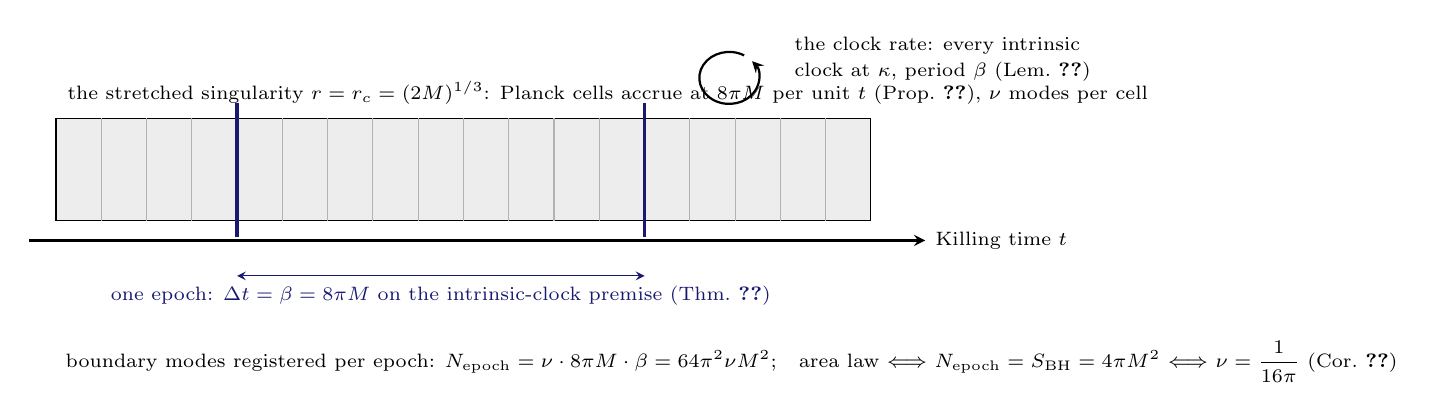
\begin{tikzpicture}[xscale=1.15, yscale=1.0]
  % the conveyor: the stretched-singularity cylinder unrolled, t horizontal
  \draw[-stealth, thick] (-0.3, 0) -- (9.6, 0) node[anchor=west, font=\scriptsize] {Killing time $t$};
  % cell band
  \fill[gray!14] (0, 0.25) rectangle (9.0, 1.55);
  \draw (0, 0.25) rectangle (9.0, 1.55);
  \foreach \x in {0.5,1.0,...,8.5} \draw[gray!60] (\x, 0.25) -- (\x, 1.55);
  \node[font=\scriptsize, anchor=south west] at (0.02, 1.6)
    {the stretched singularity $r = r_c = (2M)^{1/3}$: Planck cells accrue at $8\pi M$ per unit $t$ (Prop.\ \ref{prop:volume}), $\nu$ modes per cell};
  % epoch window
  \draw[very thick, MidnightBlue] (2.0, 0.05) -- (2.0, 1.75);
  \draw[very thick, MidnightBlue] (6.5, 0.05) -- (6.5, 1.75);
  \draw[stealth-stealth, MidnightBlue] (2.0, -0.45) -- (6.5, -0.45)
    node[midway, below, font=\scriptsize] {one epoch: $\Delta t = \beta = 8\pi M$ on the intrinsic-clock premise (Thm.\ \ref{thm:epoch})};
  % counts
  \node[font=\scriptsize, anchor=north west, align=left] at (0.0, -1.15)
    {boundary modes registered per epoch: $N_{\mathrm{epoch}} = \nu \cdot 8\pi M \cdot \beta = 64\pi^2 \nu M^2$;\quad
     area law $\Longleftrightarrow$ $N_{\mathrm{epoch}} = \SBH = 4\pi M^2$ $\Longleftrightarrow$ $\nu = \dfrac{1}{16\pi}$ (Cor.\ \ref{cor:holographic})};
  % clock annotation
  \draw[-stealth, thick] (7.6, 2.35) arc (60:400:0.33);
  \node[font=\scriptsize, anchor=west] at (8.05, 2.3)
    {\shortstack[l]{the clock rate: every intrinsic\\ clock at $\kappa$, period $\beta$ (Lem.\ \ref{lem:inventory})}};
\end{tikzpicture}}
\caption{The counting geometry in one picture. The stretched singularity accrues Planck cells at $8\pi M$ per unit Killing time, exactly at leading order in $r_c/2M$, under the framework's own curvature cutoff (Proposition \ref{prop:volume}), carrying $\nu$ boundary modes per cell (Theorem \ref{thm:count}). Every intrinsic clock of the boundary modes runs at the modular rate, period $\beta = 8\pi M$ (Lemma \ref{lem:inventory}); on the flagged premise that the counted epoch is intrinsic, the epoch is that period (Theorem \ref{thm:epoch}), and the area law becomes the single falsifiable statement $\nu = 1/16\pi$ in the 1-nat convention: one boundary-mode fermion per four Planck cells of horizon area per modular period, $N_{\mathrm{epoch}} = \SBH$ up to the absorbed per-mode $\ln 2$ (Corollary \ref{cor:holographic}). The naive $\nu = 1$ reading overshoots by exactly $16\pi$, the horizon-area coefficient.}
\label{fig:conveyor}
\end{figure}

\begin{remark}[The circularity fence]\label{rem:fence}
T5's capacity statement (the Page-curve computation) \emph{cites} the count of Section \ref{sec:count} and the area-law condition under test; any derivation of the epoch routed through the Page-curve or eviction computation therefore proves the prediction from itself, and is excluded. Admissible derivations of $\nu = 1/16\pi$ in the 1-nat convention, $\nu = 1/(16\pi\ln 2)$ in the capacity convention (Remark \ref{rem:nu}), must come from the structure of the boundary modes themselves (a calibration principle on the exceptional set of the weighted completion, Section \ref{subsec:calibration}, or the slice-to-epoch aggregation of Section \ref{sec:sphere}); the fence is part of what makes the prediction falsifiable, and the failed direct aggregations recorded in Section \ref{sec:sphere} show that it excludes real candidates.
\end{remark}

\begin{remark}[Point of contact: what kind of statement this is]\label{rem:epochtouch}
The step of Theorem \ref{thm:epoch} is the framework's version of a familiar holographic practice: when a quantity is conditional on a regulator, derive the regulator from the system's own modular structure. The coherence checks are threefold: the causal epoch of Fact \ref{fact:ledger} is $O(M)$ with an identified logarithm, matching the modular period's scale; the count's rate is set by the horizon's own temperature, $dN/dt = \nu/\TH$; and the epoch three-volume comes out as $\beta^2\lP$, modular up to a single Planck factor. None of the three is a proof of (IC), and the third is the weakest, its power of $\lP$ the residue of geometry; together they are why the premise is worth flagging rather than discarding.
\end{remark}


\subsection{The calibration factorised, and the quarter examined}\label{subsec:calibration}

Theorem \ref{thm:epoch} leaves one number, and Fact \ref{fact:capacity} places it at the exceptional set of the weighted completion. The geometry paper's weighted limit holds at transport level along every tangential curve of fixed Hubble-normalised length for the whole admissible class (the metrics of \cite[Def.~5.5]{ButlerT6}, whose Kasner-type exponents satisfy $\sum_i p_i^2 = 1$, as Schwarzschild's $(-\tfrac13, \tfrac23, \tfrac23)$ do), and at Schwarzschild the $\varphi$-lines converge with rate $\tau^{1/3}$ and the boundary data are regular by symmetry \cite[\S 5.5]{ButlerT6}; the prediction is stated at Schwarzschild, where no billiard arises. So no analytic obstacle remains between the framework and $\nu$; what remains is a calibration principle, carried by this paper (Remark \ref{rem:nu}), and the results below say what it must produce: the required thinning factorises; exactness excludes the cutoff from the count and narrows the normalisation to two cutoff-free scales, the horizon $r_h$ and $r_* = M$; one tick per modular period is (IC) read as a counting rule; and the residue is Bekenstein-Hawking's quarter, which in the one convention that compares an entropy with an entropy is $1/(4\ln 2)$, unreachable by any counting rule whose residue is rational ($k = 0$ in Proposition \ref{prop:norecount}) and, conditionally on the expected algebraic independence of $\pi$ and $\ln 2$, by any counting rule at all.

\begin{fact}[Imported: the collar's coframe at the exceptional set, and the helicity lift]\label{fact:collarframe}
In units $2M = 1$ the weighted coframe of the Schwarzschild interior carries the weights $r^{1/2}$ on $\sqrt{A}\,dt$ and $r^{-1}$ on $r\,d\theta$, $r\sin\theta\,d\varphi$: these are the Kasner exponents $(-\tfrac13, \tfrac23, \tfrac23)$ of the proper-time variable $\tau \propto r^{3/2}$ rewritten in the variable $r$, where they read $(-\tfrac12, 1, 1)$, normalised to one at $r = r_h$; the horizon-normalised coframe on the exceptional set is therefore $(dt,\ r_h\,d\theta,\ r_h\sin\theta\,d\varphi)$ exactly, $(r^{1/2}\sqrt{A})^2 = 1 - r \to 1$ and $r^{-1}\cdot r = 1$. In the Hawking paper's lift, each channel $(\omega, \ell, m, s)$ of the near-horizon reduction is one two-dimensional mode, and the two helicities of a massless species are two channels at distinct homogeneities $-2s - 2$ ($-4$ and $0$ for the photon, $-6$ and $+2$ for the graviton); the channel identification is that paper's joint J3, its one modelling joint, which it assigns to this paper as an open successor problem, so the lift enters here at modelling tier and not at theorem tier. \emph{Provenance:} \cite[Lemmas 5.1 to 5.3, Def.~5.5]{ButlerT6} and \cite[Thm.~8.16]{ButlerT4} for the weights; \cite[Fact~5.1, Prop.~5.2, Assembly~5.3]{ButlerT7} for the lift, Assembly 5.3 there itemising J3 as modelling.
\end{fact}

\begin{proposition}[The exact factorisation of the thinning]\label{prop:factor}
In Planck units, with $r_h = 2M$, $A = 4\pi r_h^2 = 16\pi M^2$, $\beta = 8\pi M$ and $\SBH = A/4$:
\begin{enumerate}
\item[(i)] the slice count per unit Killing time is $8\pi M = 4\pi r_h = A/r_h$, at leading order in $r_c/2M$;
\item[(ii)] the slice count per modular period is $N_{\mathrm{slice}} = 64\pi^2 M^2$ and $N_{\mathrm{slice}}/\SBH = 16\pi$, at the same order;
\item[(iii)] $16\pi = (\beta/r_h) \times (A/\SBH) = 4\pi \times 4$, and the first factor is universal for Schwarzschild, $\beta/r_h = 2\pi/(\kappa r_h) = 4\pi$ with $\kappa = 1/(2r_h)$.
\end{enumerate}
\end{proposition}

\begin{proof}
(i) and (ii) are Proposition \ref{prop:volume} and Theorem \ref{thm:epoch}'s numbers multiplied, and inherit Proposition \ref{prop:volume}'s leading-order qualifier, the neglected factor being $\sqrt{1 - r_c/2M}$; (iii) is arithmetic, exact, $\beta/r_h = 8\pi M/2M = 4\pi$ and $A/\SBH = 4$. The script performs all of it as exact monomials in $\pi$ and $M$.
\end{proof}

The two factors are different kinds of question. The $4\pi = \beta/r_h$ measures the modular period in units of the horizon's own Killing time scale; it is what disappears if the $t$-direction of the exceptional set is counted \emph{once per modular period} instead of once per slice cell, which is (IC) read as a counting rule. The remaining $4$ is $A/\SBH$, Bekenstein-Hawking's quarter, which falls on the sphere factor when the sphere is counted at horizon normalisation.

\begin{proposition}[The candidate principles and their yields]\label{prop:yields}
Let a calibration principle be a rule assigning to the exceptional set $E = \{\tau = 0\} \times \R_t \times S^2$ a count of boundary-mode fermions per modular period. Then:
\begin{enumerate}
\item[(P1)] \emph{one fermion per Planck cell of the slice} returns $N_{\mathrm{epoch}} = 16\pi\,\SBH$, and the coefficient is scheme-bound: the slice count scales as $c_0^{3/2}$, so the proper-time scheme returns exactly $\tfrac32$ times the curvature scheme's count and the Kretschmann scheme $12^{1/4}$ times it, an irrational multiple;
\item[(P3)] \emph{one fermion per Planck cell of the sphere at horizon normalisation, once per modular period} returns $N_{\mathrm{epoch}} = A = 4\,\SBH$, independently of the cutoff scheme, because the horizon-normalised coframe on $E$ is exactly $(dt,\ r_h\,d\theta,\ r_h\sin\theta\,d\varphi)$ (Fact \ref{fact:collarframe});
\item[(P2)] \emph{fundamentals per sphere aggregated over the epoch} breaks the $M$-scaling (Proposition \ref{prop:n2}).
\end{enumerate}
\end{proposition}

\begin{proof}
(P1): $N_{\mathrm{slice}}$ of Proposition \ref{prop:factor}; the slice volume per unit $t$ is $4\pi r_c^2\sqrt{2M/r_c} = 4\pi\sqrt{2M}\,r_c^{3/2}$, proportional to $c_0^{3/2}$ (Lemma \ref{lem:scheme}); the script computes $(c_0/2^{1/3})^{3/2}$ on the prime factorisations, $2^{-1}3^{1} = \tfrac32$ for the proper-time scheme and $2^{1/2}3^{1/4} = 12^{1/4}$ for Kretschmann. (P3): the weights of Fact \ref{fact:collarframe}, with $(r^{1/2}\sqrt A)^2 = r(1/r - 1) = 1 - r$ evaluated at $r = 0$ by the script; the sphere of radius $r_h$ has $A$ Planck cells, and one per period gives $A$. (P2) is Proposition \ref{prop:n2}.
\end{proof}

\begin{proposition}[Exactness excludes cutoff dependence]\label{prop:exactnorm}
Suppose a calibration principle returns $N_{\mathrm{epoch}} = \SBH = 4\pi M^2$ exactly and its count is a monomial $c\,\pi^p M^m$ in the geometric data of the interior with $c$ rational. Then the count cannot depend on the stretched radius $r_c$: any dependence on $r_c$ through a power $r_c^a$, $a \neq 0$, carries the scheme constant $c_0^a$, which differs between the three schemes for every real $a \neq 0$ and, for rational $a$, is irrational for the Kretschmann scheme whenever $a \notin 6\mathbb{Z}$. The principle must therefore be normalised at a scale the interior fixes without a cutoff. Exactness does not choose that scale: the interior fixes the horizon $r_h = 2M$, at which the sphere carries $A = 4\,\SBH$ cells and the count is $\SBH$ with the residue $\tfrac14$ on the cells (Proposition \ref{prop:residue}(i)), and it fixes equally the rational multiple $r_* = M = r_h/2$, at which the sphere carries $4\pi M^2 = \SBH$ cells and the residue is $1$. Which of the two a principle should mean is not decided here.
\end{proposition}

\begin{proof}
$c_0^a$ for the three schemes is $2^{a/3}$, $2^{2a/3}3^{a/6}$, $2^{-a/3}3^{2a/3}$; their ratios $2^{a/3}3^{a/6}$ and $2^{-2a/3}3^{2a/3}$ are not $1$ for real $a \neq 0$, so a count carrying $r_c^a$ takes different values in different schemes, and a scheme-dependent count cannot equal the scheme-independent $\SBH$ in all of them; for rational $a$ the Kretschmann constant $48^{a/6} = 2^{2a/3}\,3^{a/6}$ is rational exactly when both exponents are integers, that is when $a \in 6\mathbb{Z}$, and is otherwise irrational (at $a = 3/2$, for instance, it is $2\cdot 3^{1/4}$). The Schwarzschild interior has one dimensionful parameter, $M$, so a cutoff-free radius is a fixed multiple of $M$; the horizon is the distinguished one, with residue $\tfrac14$, and $r_* = M$ is the one at which the residue is $1$, the sphere's cell count there being $\SBH$ itself; the script displays both as arithmetic. The argument excludes the cutoff; it does not rank the two.
\end{proof}

\begin{proposition}[Pair, mode, qubit: one object]\label{prop:pair}
The tower's ladder pair $(v_i, w_i)$, the singularity paper's ``fermionic mode'', and the ``one ladder pair per point of the exceptional set'' of Fact \ref{fact:capacity} are the same object: one creation and one annihilation operator, a two-dimensional state space, one qubit, maximal entropy $\ln 2$ nats. In particular $\Cl(2,4)$ carries exactly two such pairs, its Witt index, and the count of pairs is the count of modes: no factor of two enters between the tower and this paper's count.
\end{proposition}

\begin{proof}
The tower's relations \cite[Prop.~4.1]{ButlerT3} are the CAR of $k$ modes with $v_i$ the creation and $w_i$ the annihilation operator of mode $i$, each mode's algebra $\Mat_2$ with the two-dimensional Fock space $\{|0\rangle, v_i|0\rangle\}$, one qubit per rung \cite[Thm.~4.2]{ButlerT3}; the singularity paper's per-mode capacity $\ln 2$ is the maximal entropy of that two-state system; the corank statement counts these pairs. The script realises two pairs in $\Cl(2,4)$ as $v_i = \tfrac12(e_a + e_b)$, $w_i = \tfrac12(e_a - e_b)$ on two orthogonal hyperbolic planes and checks all ten anticommutation relations exactly; that no third pair exists is the capacity theorem \cite[Thm.~4.3]{ButlerT3}.
\end{proof}

\begin{proposition}[The residue in each convention]\label{prop:residue}
Write the epoch count as $N_{\mathrm{epoch}} = \kappa_c \times A \times 1$, horizon-normalised sphere cells times one tick per modular period, with $\kappa_c$ the dimensionless \emph{calibration residue}, a symbol distinct from the surface gravity $\kappa$ of Section \ref{sec:setting}. Then:
\begin{enumerate}
\item[(i)] in the 1-nat convention of this paper, $N_{\mathrm{epoch}} = \SBH$ gives $\kappa_c = \SBH/A = \tfrac14$;
\item[(ii)] in the capacity convention of the singularity paper, $N_{\mathrm{epoch}}\ln 2 = \SBH$ gives $\kappa_c = 1/(4\ln 2)$: one boundary mode per $4\ln 2$ Planck areas of horizon per modular period, which is one mode per Bekenstein-Mukhanov area quantum \cite{BekensteinMukhanov1995};
\item[(iii)] the two differ by exactly $\ln 2$, and only (ii) compares an entropy with an entropy: a fermionic mode carries at most $\ln 2$ nats, so the 1-nat convention credits each mode with more entropy than it can hold, and the exact ``$16\pi$'' of Theorem \ref{thm:epoch} is a property of that convention, the physical thinning being $16\pi\ln 2$;
\item[(iv)] one boundary mode registers one helicity: by Fact \ref{fact:collarframe} the two helicities of a massless species are two channels of the lift, so the capacity per boundary mode is $\ln 2$ and not $2\ln 2$, and $\kappa_c$ is $1/(4\ln 2)$, not $1/(8\ln 2)$.
\end{enumerate}
\end{proposition}

\begin{proof}
(i) and (ii) are $N_{\mathrm{epoch}}/A$ with $N_{\mathrm{epoch}}$ read off Corollary \ref{cor:holographic}(2) in each convention: $N_{\mathrm{epoch}} = \SBH = 4\pi M^2$ in the 1-nat convention and $N_{\mathrm{epoch}} = \SBH/\ln 2$ in the capacity convention (the $\ln 2$ of Remark \ref{rem:nu}), divided by $A = 16\pi M^2$; the script performs them as exact monomials in $\pi$ and $M$ with $\ln 2$ a formal indeterminate. (iii): the maximal entropy of a two-dimensional state space is $\ln 2$, the entropy of the maximally mixed state, and $\ln 2 < 1$; the singularity paper already compares $C = N\ln 2$ with $\SBH$ for this reason \cite[Prop.~10.7]{ButlerT5}, and Remark \ref{rem:nu} records the factor. (iv) is a reading of the lift at the level of its channel identification, its modelling step: the homogeneities $-2s - 2$ at $s = \pm 1, \pm 2$ are $-4, 0, -6, +2$, pairwise distinct, so no single channel contains both helicities; the script checks the table.
\end{proof}

\begin{proposition}[No recount reaches the quarter]\label{prop:norecount}
Let a counting rule assign to the exceptional set a tally that is a rational number of modes per cell, with cells whose areas are rational multiples of integer powers of $\pi$ in Planck units, over a rational number of ticks per modular period. Then its residue $\kappa_c$ is a rational multiple of an integer power of $\pi$, $\kappa_c = q\pi^k$ with $q \in \mathbb{Q}$ and $k \in \mathbb{Z}$. In the capacity convention the target is $\kappa_c = 1/(4\ln 2)$; equality would require $\pi^k\ln 2 \in \mathbb{Q}$, which is false for $k = 0$, $\ln 2$ being transcendental \cite[Thm.~1.4]{Baker1975}, so no rule with $k = 0$ reaches the target; for $k \neq 0$ it would contradict the expected algebraic independence of $\pi$ and $\ln 2$, which is not a theorem, so the exclusion of rules with $k \neq 0$ is conditional on that independence. In the 1-nat convention the target $\kappa_c = \tfrac14$ is rational, and the natural rules of Proposition \ref{prop:yields} return $\kappa_c = 4\pi$ (P1), $\kappa_c = 1$ (P3) and a broken scaling (P2), none of them $\tfrac14$.
\end{proposition}

\begin{proof}
A product and quotient of rational multiples of integer powers of $\pi$ is one, which is the closure the script checks on the rule's three factors. $1/(4\ln 2) = q\pi^k$ with $q$ rational gives $\pi^k\ln 2 = 1/(4q)$ rational; at $k = 0$ this says $\ln 2$ is rational, contradicting its transcendence (Hermite-Lindemann, an import, not scripted). The residues of the natural rules are Proposition \ref{prop:yields}'s yields divided by $A$: $16\pi\,\SBH/A = 4\pi$ and $A/A = 1$.
\end{proof}

\begin{remark}[The prediction, restated]\label{rem:betrestated}
Propositions \ref{prop:factor} to \ref{prop:norecount} reduce the calibration to the form
\[
N_{\mathrm{epoch}} \;=\; \kappa_c \times (\text{horizon-normalised sphere cells}) \times (\text{one tick per modular period}),
\]
with the normalisation narrowed to two cutoff-free scales by exactness ($r_h$, or $r_* = M$, Proposition \ref{prop:exactnorm}), one tick per period being (IC) read as a counting rule, and $\kappa_c$ the residue. The residue is not an artefact of the counting conventions: the chain from tower to count carries no hidden factor of two (Proposition \ref{prop:pair}); the helicity clause is closed at the tier of the lift's modelling joint J3 (Proposition \ref{prop:residue}(iv), Fact \ref{fact:collarframe}), not at theorem tier; and in the one convention with physical content the residue is $1/(4\ln 2)$, which no recount of the exceptional set with a rational residue ($k = 0$) produces, and, conditionally on the expected algebraic independence of $\pi$ and $\ln 2$, no recount with $k \neq 0$ either (Proposition \ref{prop:norecount}). The prediction's declared form is therefore: \emph{the boundary mode space registers one mode per Bekenstein-Mukhanov area quantum of horizon per modular period}, $\nu = 1/(16\pi\ln 2)$ in the capacity convention, and deriving that is equivalent to deriving Bekenstein-Hawking's quarter. Arithmetically $\kappa_c = \tfrac14$ in the 1-nat convention is horizon normalisation replaced by normalisation at $r_* = r_h/2 = M$, since $4\pi M^2 = \SBH$; whether that radius means anything is not decided here. The $16\pi$ of Theorem \ref{thm:epoch} stands as the convention-dependent form of the same statement.
\end{remark}

% === Section 5 (M3): the sphere ===
\section{The transverse sphere from the boundary modes}\label{sec:sphere}

The count of Section \ref{sec:count} used the metric slice geometry. This section derives the transverse angular geometry from the correlation structure itself, completing a sequence whose first two steps are standard modular theory, and then runs the quantitative checks: one exact agreement, and two instructive failures.

\begin{fact}[Imported: time and the plane from modular data]\label{fact:modular2d}
The modular flow of a wedge algebra in the vacuum implements the boost: the timelike direction is recoverable from modular data (Bisognano-Wichmann). One half-sided modular inclusion recovers the two-dimensional conformal structure (Wiesbrock). \emph{Provenance:} \cite{BisognanoWichmann1976} (the duality theorem) and \cite{Wiesbrock1993} (the main theorem); both at assembly level for the present use.
\end{fact}

\begin{proposition}[The boundary mode space as matrix]\label{prop:matrix}
Let the boundary mode space carry $n$ completed pairs, $n$ counted after the completion's doubling (each mode with its adjoined partner). The gauge-invariant bilinears $E_{ij} := \psi_i^\dagger \psi_j$ satisfy $[E_{ij}, E_{kl}] = \delta_{jk}E_{il} - \delta_{li}E_{kj}$ (the $\mathfrak{gl}(n)$ relations, an instance of the CAR bilinear commutator), preserve the one-particle subspace, and restrict on it to the full matrix algebra: $E_{ij}|_{\text{one-particle}} = $ the matrix unit $e_{ij}$, so the associative algebra they generate restricts onto $\Mat_n$. The doubling the completion forces is exactly what turns a tower of modes into a matrix; and matrices can be spheres.
\end{proposition}

\begin{proof}
The commutator identity is the bilinear computation used already in \cite[Prop.~6.1]{ButlerT7} (there for the currents; here for general index pairs): $[\psi_i^\dagger\psi_j, \psi_k^\dagger\psi_l] = \delta_{jk}\psi_i^\dagger\psi_l - \delta_{li}\psi_k^\dagger\psi_j$ from the CAR. Each $E_{ij}$ maps the one-particle subspace $\operatorname{span}\{\psi_k^\dagger|0\rangle\}$ to itself, acting as $e_{ij}$ ($E_{ij}\psi_k^\dagger|0\rangle = \delta_{jk}\psi_i^\dagger|0\rangle$); the matrix units generate $\Mat_n$, so the restriction map is onto. The doubling is what supplies the complex structure: each real mode with its adjoined partner supplies the complex $\psi_i, \psi_i^\dagger$ from which the gauge-invariant $E_{ij}$ are built; real Clifford directions alone give the orthogonal bilinears, and it is the pairing that produces $\mathfrak{gl}(n)$. The script checks the commutator table and the one-particle action exactly on a five-mode instance.
\end{proof}

\begin{fact}[Imported: Kostant, Madore, and the $\mathfrak{sl}_2$ partition data]\label{fact:kostant}
(i) Embeddings of $\mathfrak{sl}_2$ into $\mathfrak{gl}_n$ are classified, up to conjugation, by the partition of $n$ given by the restriction of the defining representation; the \emph{principal} embedding is the one with a single part (the irreducible $n$-dimensional representation), and it is essentially unique. (ii) For the principal embedding the adjoint decomposition of $\Mat_n$ is multiplicity-free: $\Mat_n \cong \bigoplus_{\ell=0}^{n-1}(2\ell + 1)$, one spin-$\ell$ multiplet for each $\ell < n$ (Kostant). (iii) $\Mat_n$ with this $\mathfrak{su}(2)$ structure is Madore's fuzzy sphere, whose large-$n$ limit is the round $S^2$ \cite{Madore1992}, radius excluded: the radius is scale. \emph{Provenance:} \cite{Kostant1959} (the principal three-dimensional subgroup and the multiplicity-free adjoint decomposition) and \cite{Madore1992} (the fuzzy sphere and its large-$n$ limit); the $\mathfrak{sl}_2$ classification is classical representation theory.
\end{fact}

\begin{principle}[Indifference, structural premise of the series]\label{prin:indiff}
The framework forbids uncaused structure: a construction may not carry distinctions (partitions, assignments, orderings) that nothing in the framework determines. \emph{Provenance and level:} this is the structural principle used to order the family faces, applied here at the declared level; it is a premise of the derivation below, not a theorem, and is flagged as such.
\end{principle}

\begin{theorem}[Principality from indifference: the sphere]\label{thm:sphere}
Under Principle \ref{prin:indiff}, the $\mathfrak{su}(2)$ structure carried by the matrix algebra of the boundary modes (Proposition \ref{prop:matrix}) is the principal embedding, uniquely: a non-principal embedding decomposes the $n$ modes into invariant blocks, a partition whose sizes and assignments nothing in the framework causes (Fact \ref{fact:kostant}(i)), and indifference forbids exactly such uncaused data; the principal embedding is the unique one carrying no partition data, its internal distinctions forced by the algebra once conjugation-gauge is fixed. Consequently the bilinear sector of the boundary modes is canonically Madore's fuzzy sphere, and its large-$n$ limit is the round transverse $S^2$, radius state-side: three of the four emergent dimensions now rest on the correlation structure (time and the plane from Fact \ref{fact:modular2d}, the sphere from this theorem), the fourth being scale. The conclusion is conditional on Principle \ref{prin:indiff} wherever this theorem is cited.
\end{theorem}

\begin{proof}
The mathematical content is the classification of Fact \ref{fact:kostant}(i): the conjugacy classes of embeddings are the partitions of $n$, and every class except $(n)$ carries a nontrivial partition; the selection is then the application of the Principle, whose level is declared there. Uniqueness up to conjugation is Kostant's, and conjugation is the gauge freedom the statement fixes. The multiplicity-free decomposition and the fuzzy-sphere reading are Fact \ref{fact:kostant}(ii)-(iii). The script exhibits the distinction concretely at $n = 3$: the principal $\mathfrak{sl}_2$ (an exact integer triple) has adjoint decomposition of $\Mat_3$ with exactly three irreducible summands of dimensions $1 + 3 + 5 = 9$ (kernel of $\operatorname{ad}_e$ of dimension three), while a non-principal block embedding has a larger highest-weight space (multiplicities), verifying the partition-data diagnosis in exact arithmetic.
\end{proof}

\begin{proposition}[Consistency with the CAR construction, and the I-state's insensitivity]\label{prop:consistency}
Three checks, each at its level. (i) \emph{Assembly:} the near-horizon reduction delivers one field per $(\ell, m)$ with $m$-independent dynamics, so the modular flow acts as a scalar on each multiplet and centralises the $\mathfrak{su}(2)$: the sphere's symmetry commutes with the clock. (ii) \emph{Proved:} the mixed bilinears of Proposition \ref{prop:matrix} are ordinary gauge-invariant CAR bilinears of the observable algebra: no operator outside the algebra of the boundary modes themselves is invoked. (iii) \emph{Proved, within the quasi-free setting:} the I-state with multiplet-degenerate frequencies is invariant under every gauge Bogoliubov transformation of the complexified one-particle space commuting with the one-particle Hamiltonian, in particular under all embedded $SU(2)$ actions: for a quasi-free state whose symbol is a function of the one-particle Hamiltonian, $\Lambda = g(h)$, and a unitary $U$ on the one-particle space with $UhU^* = h$, the transformed state has symbol $U\Lambda U^* = Ug(h)U^* = g(h) = \Lambda$, the same state. The I-state is embedding-insensitive: it neither selects nor obstructs the sphere. This diagonality is the sphere's side of the orthogonality no-go carried by the action paper T10 \cite{ButlerT10}: the state is insensitive to space for the same reason the gravitational sector leaves no mark on it; the full development of that identity is that paper's task (shared between the two papers).
\end{proposition}

\begin{proof}
(i) is the standard reduction, imported and flagged as modelling in the manner of \cite[Rem.~4.5]{ButlerT7}. (ii) is inspection of Proposition \ref{prop:matrix}. (iii) is the displayed two-line computation, plus the fact that a gauge-invariant quasi-free state is determined by its symbol (\cite[Fact 3.3]{ButlerT7}, Araki); the script verifies an $SU(2)$-rotation instance on a degenerate three-mode multiplet exactly.
\end{proof}

\begin{proposition}[The per-slice verification, and the two failed aggregations]\label{prop:n2}
Let $n$ be the linear size of the slice's matrix algebra. Then:
\begin{enumerate}
\item \emph{(The slice check, exact in scaling.)} Matching the fuzzy operator dimension to the slice sphere's Planck-cell count sets $n^2 = 4\pi r_c^2 = 4\pi(2M)^{2/3}$ to leading order ($n$ is an integer matrix size and the right side transcendental; what the match fixes exactly is the $M^{2/3}$ scaling): the fuzzy count reproduces, from the matrix side, exactly the sphere-only case of Proposition \ref{prop:unique}, its $M^{2/3}$ scaling. The fuzzy geometry and the metric geometry agree slice by slice.
\item \emph{(Operator-cell aggregation fails, by exactly the area coefficient.)} Counting one boundary-mode fermion per operator cell of the epoch volume is the $\nu = 1$ reading, which overshoots $N_{\mathrm{epoch}} = \SBH$ by exactly $16\pi$ (Corollary \ref{cor:holographic}(3)): the required thinning is the horizon-area coefficient itself.
\item \emph{(Fundamental-per-slice aggregation breaks the scaling.)} Counting $n \propto M^{1/3}$ fundamentals per sphere and aggregating over the epoch's spheres (the slice volume of Proposition \ref{prop:volume} contains $8\pi M/4\pi r_c^2 = (2M)^{1/3}$ spheres per unit Killing time) gives
\[
N_{\mathrm{fund}} \;\propto\; M^{1/3}\cdot M^{1/3}\cdot \Delta t \;\propto\; M^{5/3} \quad (\Delta t \sim M),
\]
which breaks the area scaling altogether.
\end{enumerate}
Both direct aggregation rules fail, so the slice-to-epoch aggregation is the weighted completion's task: derive $N_{\mathrm{epoch}} = \SBH$, or refute the intrinsic-clock premise.
\end{proposition}

\begin{proof}
All three clauses are exact exponent arithmetic, checked by the script: (1) $4\pi r_c^2$ with $r_c = (2M)^{1/3}$; (2) is Corollary \ref{cor:holographic}(3); (3) multiplies the displayed factors, with the spheres-per-unit-time count $8\pi M / 4\pi(2M)^{2/3} = 2M/(2M)^{2/3} = (2M)^{1/3}$.
\end{proof}

% === Section 6 (M4): dynamics ===
\section{Scrambling, and the return delay}\label{sec:dynamics}

T5's eviction dynamics is a rate model, and its instant information return was flagged there as the rate model's artefact. This section supplies the internal timescales of the boundary modes at the same declared tier: a rate model whose clock, unlike its couplings, is a theorem.

\begin{assembly}[The spreading law, and the chaos bound saturated]\label{asm:spreading}
Three framework-internal facts fix the window's internal dynamics. First, the intrinsic flows of a Clifford boundary-mode algebra are bivector-generated, quadratic in the pair operators (Lemma \ref{lem:inventory}(i)). Second, the distinguished bivector flow is the boost (Fact \ref{fact:inventory}). Third, the boost is the translation clock of the window itself: the Killing flow that displaces modes along the window is the boost at rate $\kappa$, with the accrual rate of Theorem \ref{thm:count}. Boost-hyperbolic one-body dynamics expands operator amplitudes as $e^{\kappa t}$, so support deposited on a single mode spans the $N$-mode window at
\[
t_* \;=\; \kappa^{-1}\ln N \;=\; \frac{\beta}{2\pi}\,\ln S :
\]
the fast-scrambling law, with the logarithm the signature of hyperbolic dynamics rather than an assumption. In particular the boundary mode space saturates the Maldacena-Shenker-Stanford chaos bound \emph{by construction}: every intrinsic clock it has runs at the modular rate, and the expansion rate is exactly $2\pi T$. \emph{Tier, declared:} what is derived is the free-fermion operator-spreading timescale under a generic quadratic coupling, in the rate-model normalisation; genuine chaotic saturation beyond free-fermion spreading is open, and is named as such in Section \ref{sec:scope}.

\smallskip
\noindent\emph{The derivation, step by step.} The inventory clauses are Lemma \ref{lem:inventory} (proved) and its import (Fact \ref{fact:inventory}). The expansion computation: a quadratic generator containing the boost scales ladder operators by $e^{\pm\kappa t}$ (Fact \ref{fact:inventory}'s weight clause, exponentiated), so under a generic quadratic coupling the amplitude reaching a mode at mode distance $d$ grows as $e^{\kappa t}$ against an initial suppression of order $1/N$; support spans all the boundary modes when $e^{\kappa t} \sim N$, i.e.\ at $t_* = \kappa^{-1}\ln N$, and $N \sim S$ over an epoch of order $M$ (Proposition \ref{prop:arealaw}). The identification $\kappa^{-1} = \beta/2\pi$ is arithmetic ($\beta = 2\pi/\kappa$), checked by the script along with the Schwarzschild value $\beta/2\pi = 4M$. The MSS statement that no system exceeds the growth rate $2\pi T$ is the point of contact \cite{MSS2016}: a system all of whose clocks run at exactly that rate saturates it if it scrambles at all, which is the construction's content.
\end{assembly}

\begin{assembly}[The return delay: the scrambling log recovered]\label{asm:delay}
In the rate model, deposited information cannot return before the dwell time of the window (the epoch of Section \ref{sec:epoch}, the correct power of $M$); and charging the window-internal re-encoding at the framework's causal rate (one pairwise operation per boost e-fold $\kappa^{-1}$ per mode, spreading epidemically over the $N \sim S$ modes) requires of order $\ln S$ rounds of duration $\beta/2\pi$, giving a return delay
\[
T_{\mathrm{return}} \;\approx\; \frac{\beta}{2\pi}\,\ln S \;=\; 4M\,\ln S :
\]
the fast-scrambling time \cite{HaydenPreskill2007, SekinoSusskind2008}, recovered from the framework's own clock. This removes the instant-return artefact of T5's rate model; the first-principles account of the spreading exponent is Assembly \ref{asm:spreading}, and genuine chaotic dynamics beyond it remains open.

\smallskip
\noindent\emph{The derivation, step by step.} The dwell floor is the epoch (Theorem \ref{thm:epoch}, conditional on (IC)); the epidemic count is the standard doubling estimate, $\log_2 S$ rounds to reach $S$ modes from one, each round one causal step of the window's clock, the $\ln 2$ absorbed into the displayed approximation; the clock and its rate are the theorems cited. The coefficient $4M$ is exact arithmetic from $\beta = 8\pi M$, script-checked.
\end{assembly}

\begin{assembly}[The no-attic route]\label{asm:noattic}
T5's eviction theorem runs on an axiom (A), that modes exiting the window deposit their correlations in the window-radiation accounting, with no third sector. The derivation route, assembled from the series' theorems: by the localisation provided by the wall results, operator-valued degrees of freedom exist within the physical closure only where division fails (the window mode space and the radiation's partner modes are the only q-number sectors) \cite[\S 5 and \S 8]{ButlerT4}, \cite[\S 10--11]{ButlerT5}; and by the iteration corollary of the tower paper T3, one ascent completes the description on the physical closure, with no further rungs demanded there \cite[Cor.~6.2]{ButlerT3}: there is no further completion in which a third sector (an attic) could lie. Hence (A)'s content reduces to the \emph{exhaustiveness} of the localisation (the no-remnant, closure-completeness claim), exactly as T5's own derivation records; that exhaustiveness remains the conjectural core, inherited and named, and this assembly's contribution is to have isolated it: everything else in (A) is theorem-backed.

\smallskip
\noindent\emph{The derivation, step by step.} A violation of (A) requires a q-number sector outside the localisation's inventory, which the cited theorems forbid on the physical closure given exhaustiveness; the three imports are cited in the statement.
\end{assembly}

\section{The observational record}\label{sec:record}

\begin{record}[The no-echo prediction, registered]\label{rec:echo}
The framework's quantum structure lies at the stretched singularity, $r_c = (2M)^{1/3}$ in Planck units: deep inside the hole, at Planck curvature, and nowhere near the horizon, which remains exactly the smooth vacuum horizon of classical general relativity (the exterior dictionary is exact, \cite[Fact 2.1]{ButlerT6}). The registered prediction: post-merger ringdown is the Kerr quasinormal spectrum of general relativity with \emph{no} modification, and in particular no echo train at the Planck-structure delay $\tau_{\mathrm{echo}} \approx 8M\ln(M/m_P)$ (the delay at which near-horizon structure at Planck distance would reflect \cite{CardosoPani2017}), of order tens to hundreds of milliseconds for stellar-mass remnants ($35$ ms at $10\,M_\odot$, $0.1$ to $0.25$ s for remnants of $30$ to $70\,M_\odot$): within the sensitivity band of existing detectors. A single statistically confirmed echo train would refute the framework's localisation of quantum structure. The prediction is stated so that it can fail.
\end{record}

\begin{record}[The catalogue, confronted]\label{rec:catalogue}
Through the fourth gravitational-wave transient catalogue (GWTC-4.0, 2025-2026: some two hundred and eighteen compact-binary candidates, with ninety-one confident signals subjected to the dedicated tests of general relativity), the echo searches comprise two families of echo waveform templates and two morphology-agnostic searches for coherent post-merger excess power, applied to the fourth observing run's events alongside all prior ones; they report no statistically significant echo train, and the early tentative claims \cite{Abedi2017} did not survive independent reanalysis \cite{Westerweck2018, GWTC4TGR2026}. The registered prediction of Record \ref{rec:echo} therefore stands consistent with every event so far analysed, across four catalogues and four search methods. \emph{Level:} observational, resting on the cited survey record as of the catalogue date; the confrontation is not closed and cannot be: it becomes more stringent with each catalogue, and the framework remains one confirmed echo train away from refutation.
\end{record}

\section{Scope, and successor problems}\label{sec:scope}

\subsection*{The levels of the results}

\emph{Proved, at the standard of \cite{ButlerT1}:} scheme robustness with exact constants (Lemma \ref{lem:scheme}); the slice volume, exact at leading order (Proposition \ref{prop:volume}); the counting theorem and the area-law equivalence (Theorem \ref{thm:count}, Proposition \ref{prop:arealaw}); the scaling uniqueness (Proposition \ref{prop:unique}); the clock inventory (Lemma \ref{lem:inventory}); the exact epoch conversion and the integer-holographic arithmetic (the displayed identities of Theorem \ref{thm:epoch} and Corollary \ref{cor:holographic}); the factorisation of the thinning, the yields of the candidate principles, the exclusion of cutoff dependence with its two remaining scales, the pair-mode-qubit identity, the residue in each convention, and the rationality closure of a counting rule's residue with its $k = 0$ case, on the imported transcendence of $\ln 2$ (Propositions \ref{prop:factor} to \ref{prop:norecount}, the helicity clause (iv) of Proposition \ref{prop:residue} at the level of the lift's modelling joint J3 and not above it); the mode-space-as-matrix proposition and the I-state's embedding-insensitivity (Propositions \ref{prop:matrix}, \ref{prop:consistency}(ii) and (iii)); the slice check and both aggregation failures (Proposition \ref{prop:n2}, clause (2) read with the epoch fixed at $\beta$).

\emph{Conditional, on named premises:} the epoch theorem on the intrinsic-clock premise (IC) (Theorem \ref{thm:epoch}, Principle \ref{prin:ic}), with the circularity fence in force (Remark \ref{rem:fence}) and with it the integer-holographic reading of Corollary \ref{cor:holographic}; the sphere theorem on the indifference principle (Theorem \ref{thm:sphere}, Principle \ref{prin:indiff}); the no-attic route on closure-completeness (Assembly \ref{asm:noattic}); the exclusion of counting rules with $k \neq 0$ in Proposition \ref{prop:norecount}, on the expected algebraic independence of $\pi$ and $\ln 2$, which is not a theorem.

\emph{Assembly and rate-model tier, declared:} the modular recovery of time and the plane (Fact \ref{fact:modular2d}); the spreading law and the return delay (Assemblies \ref{asm:spreading} and \ref{asm:delay}); the reduction clause of Proposition \ref{prop:consistency}(i).

\emph{Observational:} the registered prediction and the catalogue confrontation (Records \ref{rec:echo} and \ref{rec:catalogue}), date-stamped.

\subsection*{Successor problems}

Five, in decreasing order of urgency. (1) \emph{Produce or refute $\nu = 1/(16\pi\ln 2)$:} derive the residue $\kappa_c = 1/(4\ln 2)$, one boundary mode per Bekenstein-Mukhanov area quantum of horizon per modular period, from the structure of the boundary modes themselves, or refute (IC); the corank is settled at one \cite[\S 8.9]{ButlerT4}, the analysis of the geometry paper's weighted limit is closed at Schwarzschild \cite[\S 5.5]{ButlerT6}, exactness narrows the normalisation to two cutoff-free scales, $r_h$ or $r_* = M$ (Proposition \ref{prop:exactnorm}), one tick per period is (IC) read as a counting rule, and no recount with a rational residue ($k = 0$) reaches $\kappa_c$, nor, conditionally on the expected algebraic independence of $\pi$ and $\ln 2$, any recount with $k \neq 0$ (Proposition \ref{prop:norecount}); Corollary \ref{cor:holographic} states the target in its sharpest form ($N_{\mathrm{epoch}} = \SBH$), and Proposition \ref{prop:n2}'s failed aggregations mark two excluded routes. (2) \emph{The Kerr ring count:} repeat Section \ref{sec:count} over the ring's codimension-two, duality-fibred exceptional structure \cite[Conj.~6.6]{ButlerT6}, which will scale differently with mass and spin, testing the count against the known angular-momentum dependence of Kerr entropy. (3) \emph{Chaotic saturation beyond free-fermion spreading:} upgrade Assembly \ref{asm:spreading} from operator-spreading to genuine out-of-time-order chaos, or show that the quadratic tier of the boundary modes is where the framework's claim ends. (4) \emph{The slice-to-epoch aggregation:} a first-principles rule taking Proposition \ref{prop:n2}(1)'s slice count to the epoch count, replacing the two failed naive rules. (5) \emph{Catalogue currency:} the confrontation of Record \ref{rec:catalogue} is with a moving record, and every new observing run is a fresh test; the stance is standing, not archival.

\section{Position in the series}\label{sec:position}

This paper is T8 of the series. \emph{It relies on seven predecessors:} the primer T0 \cite{ButlerT0} and the root paper T1 \cite{ButlerT1} for the completed-pair language, the transport principle, and the standard of proof; the tower paper T3 \cite{ButlerT3} for capacity as Witt index (Fact \ref{fact:capacity}) and for the iteration corollary the no-attic route runs on (Assembly \ref{asm:noattic}); the sheaf paper T4 \cite{ButlerT4} for the wall results that localise one ladder pair per point of the blown-up singular locus, corank one under the forced weights (Fact \ref{fact:capacity}); the singularity paper T5 \cite{ButlerT5} for the counting axioms of the boundary modes, the causal epoch, the eviction dynamics, and the geometric normalisation (Facts \ref{fact:ledger} and \ref{fact:inventory}); the geometry paper T6 \cite{ButlerT6} for the curvature scale, the interior proper-time series, and the weighted completion, closed at Schwarzschild, on whose exceptional set the calibration this paper carries is to be read (Facts \ref{fact:curvature} and \ref{fact:capacity}, Remark \ref{rem:nu}); and the spectrum paper T7 \cite{ButlerT7} for the mode's modular inventory and the quasi-free calculus behind the I-state checks (Fact \ref{fact:inventory}, Proposition \ref{prop:consistency}).

\emph{Papers that rely on this one:} the singularity paper T5 \cite{ButlerT5} conditions its counting step on the epoch and density that this paper derives, quantifies, and converts into the single prediction $\nu = 1/16\pi$ in the 1-nat convention, $\nu = 1/(16\pi\ln 2)$ in T5's own capacity convention; the action paper T10 \cite{ButlerT10} imports the sphere theorem (Theorem \ref{thm:sphere}), with its indifference premise attached, and shares the sphere's orthogonality no-go (Proposition \ref{prop:consistency}); and the capstone T17 \cite{ButlerT17} tabulates this paper's claims at their tiers.

\section{Machine verification}\label{sec:verification}

The computational identities asserted in this paper are verified by \texttt{verify\_T08.py}, the script deposited with the paper \cite{ButlerVerifyT8}; it imports the series' shared exact-arithmetic library \texttt{GA.py} and runs entirely in exact arithmetic: dimensional quantities are exact monomials $c\cdot 2^a 3^b \pi^p M^e$ with rational coefficients and exponents (normalised so equal quantities have equal representations), so every scaling claim is an identity of exponents rather than a numerical estimate; the representation-theoretic and Fock computations are over the rationals. Forty-seven checks pass. Not scripted, and stated as such where they occur: the imported Facts, certified by their source papers' scripts or by the literature (Fact \ref{fact:curvature}'s displayed Kretschmann arithmetic included); the transcendence of $\ln 2$ (Hermite-Lindemann) that Proposition \ref{prop:norecount} imports, which no script certifies; the assembly steps of Section \ref{sec:dynamics} beyond their exact coefficients; and the observational Records.

The coverage, by section. \emph{The count} (Lemma \ref{lem:scheme} through Proposition \ref{prop:unique}): the three cutoff schemes solved exactly, with the constants $2^{1/3}$, $48^{1/6} = 2^{2/3}3^{1/6}$, $3^{2/3}2^{-1/3}$ and the common $M^{1/3}$ exponent; the exact slice-volume identity $4\pi r_c^2\sqrt{2M/r_c} = 8\pi M$; the rate identity $dN/dt = \nu/\TH$; the area-law equivalence at $\nu\Delta t = M/2$; and the uniqueness arithmetic, driven by the computed exponents against the admissible set (sphere-only $M^{2/3}$, fixed-radius $M^{1/2}$, the unavailable matching timescales $M^{4/3}$, $M^{3/2}$). \emph{The calibration} (Section \ref{subsec:calibration}): the factorisation $16\pi = 4\pi \times 4$ and its ingredients as exact monomials; the scheme ratios $\tfrac32$ and $12^{1/4}$ on the prime factorisations; the horizon-normalised coframe values at $r = 0$; the ten anticommutation relations of two ladder pairs in $\Cl(2,4)$; the two cutoff-free scales and their residues $\tfrac14$ and $1$; the two calibrations with $\ln 2$ a formal indeterminate; the homogeneity table of the helicity lift; the natural rules' residues $4\pi$ and $1$ against the target $\tfrac14$; and the rationality closure of a counting rule's residue on eighty rules built from the paper's objects, none reaching $1/(4\ln 2)$ as a formal expression in $\ln 2$ while one reaches $\tfrac14$ (Propositions \ref{prop:factor} to \ref{prop:norecount}; the step from the formal to the numerical exclusion at $k = 0$ is the imported transcendence). \emph{The clock inventory} (Lemma \ref{lem:inventory}): the adjoint spectra of the inventory's representatives classified exactly from their $2\times2$ rational blocks, transcribed from the proof's computation, and the same conclusions re-derived from a two-mode CAR representation built in the script (mode operators as exact Fock matrices, the pairing generators built rather than asserted, $\operatorname{ad}_X$ computed by commutator and the criterion read off it); the clock criterion run on each case (the atom, rotated-pair, opposed, common and paired boosts admitted; the compact, nilpotent, unequal-magnitude and complex-spectrum elements excluded), the pairing trichotomy certified by the sign of $cd$, and the discriminating cases $E_{11} + E_{12} - E_{21}$ (every adjoint eigenvalue of modulus one, none real: the modulus-only variant the script also runs admits it, the stated criterion excludes it) and $E_{11} + E_{12} + E_{22}$ (real adjoint eigenvalues, all nonzero of modulus one, excluded by semisimplicity alone). \emph{The epoch} (Theorem \ref{thm:epoch}, Corollary \ref{cor:holographic}): $\beta = 2\pi/\kappa = 8\pi M$; the conversion $\nu = 1/16\pi$ in the 1-nat convention; the epoch three-volume $V = 64\pi^2M^2 = \beta^2\lP$; $\nu V = 4\pi M^2 = \SBH$; and the $16\pi$ overshoot identified with the horizon-area coefficient, all as exact monomial identities, with $\SBH$ and the horizon area derived from $r_s = 2M$ and anchored by their own check rather than typed in. \emph{The sphere} (Theorem \ref{thm:sphere}, Propositions \ref{prop:matrix}, \ref{prop:consistency}, \ref{prop:n2}): an integer principal $\mathfrak{sl}_2$ triple in $\Mat_3$ with its bracket table verified exactly; the adjoint kernel of $\operatorname{ad}_e$ of dimension exactly three (multiplicity-free $1 + 3 + 5$) against dimension five for a non-principal block embedding (partition data made visible); the $\operatorname{ad}_h$ weight multiset $\{0,0,0,\pm2,\pm2,\pm4\}$; the $\mathfrak{gl}(n)$ bilinear commutator identities on the full five-mode Fock space and the one-particle restriction onto matrix units; the second-quantised rational rotation ($U$ orthogonal with entries in fifths) verified exact and particle-number preserving, the equal-occupancy quasi-free product state verified invariant under it entrywise, and a control at unequal occupancies verified to break the invariance, the degeneracy hypothesis made visible: the I-state's embedding-insensitivity certified on the state itself; the slice-count and spheres-per-time exponents, and the $M^{5/3}$ failure of fundamental-per-slice aggregation. \emph{The dynamics} (Assemblies \ref{asm:spreading} and \ref{asm:delay}): the scrambling coefficient $4M$, as the arithmetic of $\beta$ and $\kappa$ already fixed. The script exits nonzero on any failure and prints one line per check, tagged by the statement or section it certifies.

\begin{thebibliography}{99}

\bibitem{ButlerT0}
L.~Butler,
\emph{An Introduction to Geometric Algebra: A Primer for the Transport Papers},
Transport Papers T0 (2026).

\bibitem{ButlerT1}
L.~Butler,
\emph{The Transport Principle: Total Division in Clifford Algebras via Minimal Completion},
Transport Papers T1 (2026).

\bibitem{ButlerT3}
L.~Butler,
\emph{The Tower and the CAR Limit: Iterated Transport, the Frozen Clock, and Second Quantisation},
Transport Papers T3 (2026).

\bibitem{ButlerT4}
L.~Butler,
\emph{Clifford Sheaves over Degenerate Metrics: Nilpotent Ideals, One-Sided Completion, and the Exceptional Algebra},
Transport Papers T4 (2026).

\bibitem{ButlerT5}
L.~Butler,
\emph{Division by Zero at the Gravitational Singularity: The Transport Principle Applied to the Black Hole, and the Information Paradox as a Category Error},
Transport Papers T5 (2026).

\bibitem{ButlerT6}
L.~Butler,
\emph{The Geometry of the Black-Hole Interior: Where Division Fails, the Weighted Limit, and the Kerr Tests},
Transport Papers T6 (2026).

\bibitem{Baker1975}
A.~Baker,
\emph{Transcendental Number Theory},
Cambridge University Press (1975).

\bibitem{BekensteinMukhanov1995}
J.~D.~Bekenstein and V.~F.~Mukhanov,
Spectroscopy of the quantum black hole,
\emph{Phys. Lett. B} \textbf{360} (1995) 7--12.

\bibitem{ButlerT7}
L.~Butler,
\emph{Hawking Radiation from the Ledger: State, Continuum, Lift, and the Finite-Ledger Seam},
Transport Papers T7 (2026).

\bibitem{ButlerT10}
L.~Butler,
\emph{Dark Energy and the Action of Gravity: MacDowell-Mansouri, the Frozen Point, and One Way to Grip},
Transport Papers T10 (2026).

\bibitem{ButlerT17}
L.~Butler,
\emph{The Transport Programme: Method, Status, and the Falsifiable Ledger},
Transport Papers T17 (2026).

\bibitem{Bekenstein1973}
J.~D.~Bekenstein,
Black holes and entropy,
\emph{Phys.\ Rev.\ D} \textbf{7} (1973), 2333--2346.

\bibitem{Hawking1975}
S.~W.~Hawking,
Particle creation by black holes,
\emph{Commun.\ Math.\ Phys.} \textbf{43} (1975), 199--220.

\bibitem{tHooft1985}
G.~'t~Hooft,
On the quantum structure of a black hole,
\emph{Nucl.\ Phys.\ B} \textbf{256} (1985), 727--745.

\bibitem{ChristodoulouRovelli2015}
M.~Christodoulou and C.~Rovelli,
How big is a black hole?,
\emph{Phys.\ Rev.\ D} \textbf{91} (2015), 064046.

\bibitem{HaydenPreskill2007}
P.~Hayden and J.~Preskill,
Black holes as mirrors: quantum information in random subsystems,
\emph{JHEP} \textbf{0709} (2007), 120.

\bibitem{SekinoSusskind2008}
Y.~Sekino and L.~Susskind,
Fast scramblers,
\emph{JHEP} \textbf{0810} (2008), 065.

\bibitem{MSS2016}
J.~Maldacena, S.~H.~Shenker and D.~Stanford,
A bound on chaos,
\emph{JHEP} \textbf{1608} (2016), 106.

\bibitem{Kostant1959}
B.~Kostant,
The principal three-dimensional subgroup and the Betti numbers of a complex simple Lie group,
\emph{Amer.\ J.\ Math.} \textbf{81} (1959), 973--1032.

\bibitem{Madore1992}
J.~Madore,
The fuzzy sphere,
\emph{Class.\ Quantum Grav.} \textbf{9} (1992), 69--87.

\bibitem{Wiesbrock1993}
H.-W.~Wiesbrock,
Half-sided modular inclusions of von Neumann algebras,
\emph{Commun.\ Math.\ Phys.} \textbf{157} (1993), 83--92.

\bibitem{BisognanoWichmann1976}
J.~J.~Bisognano and E.~H.~Wichmann,
On the duality condition for quantum fields,
\emph{J.\ Math.\ Phys.} \textbf{17} (1976), 303--321.

\bibitem{CardosoPani2017}
V.~Cardoso and P.~Pani,
Tests for the existence of black holes through gravitational wave echoes,
\emph{Nat.\ Astron.} \textbf{1} (2017), 586--591.

\bibitem{Abedi2017}
J.~Abedi, H.~Dykaar and N.~Afshordi,
Echoes from the abyss: tentative evidence for Planck-scale structure at black hole horizons,
\emph{Phys.\ Rev.\ D} \textbf{96} (2017), 082004.

\bibitem{Westerweck2018}
J.~Westerweck et al.,
Low significance of evidence for black hole echoes in gravitational wave data,
\emph{Phys.\ Rev.\ D} \textbf{97} (2018), 124037.

\bibitem{GWTC4TGR2026}
The LIGO-Virgo-KAGRA Collaboration,
GWTC-4.0: tests of general relativity III,
preprint (2026); with the catalogue GWTC-4.0 (2025-2026).

\bibitem{ButlerVerifyT8}
L.~Butler,
\emph{verify\_T08.py: exact-arithmetic verification of the computational identities of ``Black-Hole Entropy and Scrambling''},
Python script, deposited with this paper alongside the shared library GA.py (2026).

\end{thebibliography}

\end{document}
